% Source: Graph_ML/Semi_Supervised_Graph_Learning/semi_supervised_graph_learning.tex
\begin{notechapter}
% ---- chapter-local definitions ----
\sisetup{
  table-format=1.3,
  table-number-alignment=center,
  table-auto-round,
  table-align-text-post=false
}
\lstset{
    basicstyle=\ttfamily\small,
    breaklines=true,
    columns=flexible,
    frame=single,
    numbers=left,
    numberstyle=\tiny,
    keywordstyle=\color{blue},
    commentstyle=\color{green!50!black},
    stringstyle=\color{red}
}
\definecolor{exampleblue}{RGB}{230,242,255}
\definecolor{insightgreen}{RGB}{232,245,233}
\definecolor{warningyellow}{RGB}{255,249,230}
\definecolor{labeledred}{RGB}{220,70,70}
\definecolor{labeledgreen}{RGB}{50,140,50}
\definecolor{unlabeledblue}{RGB}{144,202,249}
\definecolor{numericalbox}{RGB}{255,245,230}
\definecolor{correctcolor}{RGB}{200,230,201}
\definecolor{smoothcolor}{RGB}{187,222,251}
\definecolor{maskcolor}{RGB}{255,204,204}
\forgetenv{insightbox}\newtcolorbox{insightbox}[1][]{colback=insightgreen, 
  colframe=green!75!black, title=Key Insight, breakable, #1}
\forgetenv{warningbox}\newtcolorbox{warningbox}[1][]{colback=warningyellow, 
  colframe=orange!75!black, title=Important Note, breakable, #1}
\forgetenv{numericalexample}\newtcolorbox{numericalexample}[1][]{colback=numericalbox, 
  colframe=orange!60!black, title=Numerical Example, breakable, #1}
\forgetenv{correctionbox}\newtcolorbox{correctionbox}[1][]{colback=correctcolor,
  colframe=green!50!black, title=Correct Step, breakable, #1}
\forgetenv{smoothingbox}\newtcolorbox{smoothingbox}[1][]{colback=smoothcolor,
  colframe=blue!50!black, title=Smooth Step, breakable, #1}
\forgetenv{maskbox}\newtcolorbox{maskbox}[1][]{colback=maskcolor,
  colframe=red!50!black, title=Masked Label Prediction, breakable, #1}
\forgetcs\R\newcommand{\R}{\mathbb{R}}
\forgetcs\E\newcommand{\E}{\mathbb{E}}
\forgetcs\norm\newcommand{\norm}[1]{\left\|#1\right\|}
\forgetcs\abs\newcommand{\abs}[1]{\left|#1\right|}
\forgetcs\inner\newcommand{\inner}[2]{\langle #1, #2 \rangle}
\forgetcs\argmin\newcommand{\argmin}{\operatorname*{argmin}}
\forgetcs\argmax\newcommand{\argmax}{\operatorname*{argmax}}
\forgetcs\tr\newcommand{\tr}{\operatorname{tr}}
\forgetcs\diag\newcommand{\diag}{\operatorname{diag}}
\forgetcs\rank\newcommand{\rank}{\operatorname{rank}}
\forgetcs\sign\newcommand{\sign}{\operatorname{sign}}
\forgetcs\softmax\newcommand{\softmax}{\operatorname{softmax}}
\forgetcs\mask\newcommand{\mask}{\mathcal{M}}
\forgetcs\corr\newcommand{\corr}{\text{corr}}
\forgetcs\smooth\newcommand{\smooth}{\text{smooth}}
% -----------------------------------
\chapter{Semi-Supervised Learning on Graphs}\label{ch:semi-supervised-graphs}
\chaptersubtitle{A mathematical foundation}

\begin{abstract}
This document provides a self-contained, mathematically rigorous treatment of
semi-supervised learning on graph-structured data. Starting from first
principles, we develop all necessary background---graph Laplacians, spectral
theory, reproducing kernel Hilbert spaces, random walks---before presenting the
core methods: label propagation, label spreading, correct \& smooth, graph
regularization, graph neural networks, and self-supervised pretraining. Every
theorem is stated with precise hypotheses and proved in full (longer proofs
are deferred to appendices). Numerical examples and figures accompany all
major results. The document is designed for self-study: no concept is used
before it is defined.
\end{abstract}

\section{Introduction}

\subsection{The Semi-Supervised Learning Paradigm}

\begin{definition}[Learning Paradigms]
\label{semi-supervised-graphs:def:paradigms}
\leavevmode
\begin{enumerate}
    \item \textbf{Supervised Learning}: Given $\mathcal{D} = \{(x_i, y_i)\}_{i=1}^n$
      with all labels known, learn $f: \mathcal{X} \to \mathcal{Y}$.
    \item \textbf{Unsupervised Learning}: Given $\mathcal{D} = \{x_i\}_{i=1}^n$
      with no labels, discover structure (clusters, manifolds, etc.).
    \item \textbf{Semi-Supervised Learning}: Given labeled set
      $\mathcal{D}_L = \{(x_i, y_i)\}_{i=1}^l$ and unlabeled set
      $\mathcal{D}_U = \{x_i\}_{i=l+1}^{l+u}$ where typically $u \gg l$,
      exploit both to improve over using $\mathcal{D}_L$ alone.
\end{enumerate}
\end{definition}

\begin{insightbox}
\textbf{Why Semi-Supervised Learning Matters:}
In many domains, obtaining labels is expensive (medical diagnosis requires
expert annotations, web-page classification faces billions of pages with few
labeled), while unlabeled data is abundant and encodes the underlying data
distribution.
\end{insightbox}

\subsection{Semi-Supervised Learning on Graphs}

\begin{definition}[Semi-Supervised Graph Setting]
\label{semi-supervised-graphs:def:ssl_graph}
Let $G = (V, E, A, X, Y_L)$ where:
\begin{itemize}
    \item $V = \{v_1, \ldots, v_n\}$ is the node set ($|V|=n$)
    \item $E \subseteq \binom{V}{2}$ is the edge set (unordered pairs)
    \item $A \in \R^{n \times n}$ is the adjacency matrix
      (Definition~\ref{semi-supervised-graphs:def:adjacency})
    \item $X \in \R^{n \times d}$: row $x_i \in \R^d$ is the feature vector
      of node $v_i$ (may be absent)
    \item $Y_L$: labels for a subset $\mathcal{V}_L \subset V$ with
      $|\mathcal{V}_L| = l \ll n$
\end{itemize}
Goal: predict $\hat{y}_i \in \mathcal{Y}$ for every $i \in \mathcal{V}_U =
V \setminus \mathcal{V}_L$.
\end{definition}

\begin{assumption}[Graph Smoothness / Homophily]
\label{semi-supervised-graphs:ass:smoothness}
Connected nodes tend to share the same label: if $\{v_i, v_j\} \in E$ with
weight $A_{ij}$, the probability that $y_i = y_j$ increases with $A_{ij}$.
\end{assumption}

\begin{remark}[Homophily vs.\ Heterophily]
\label{semi-supervised-graphs:rem:heterophily}
Assumption~\ref{semi-supervised-graphs:ass:smoothness} is the \emph{homophily} regime. In
\emph{heterophilic} graphs (e.g., dating networks, protein interactions),
connected nodes tend to have \emph{different} labels. Standard methods (label
propagation, GCN) degrade under heterophily; see~\cite{semi-supervised-graphs:zhu2020beyond,semi-supervised-graphs:lim2021large} for dedicated architectures.
\end{remark}

\subsection{Transductive vs.\ Inductive Learning}

\begin{definition}[Transductive Learning]
The unlabeled set $\mathcal{V}_U$ is known at training time. The model
predicts labels for \emph{these specific nodes} and cannot handle unseen nodes.
\end{definition}

\begin{definition}[Inductive Learning]
We learn a parametric function $f_\theta$ applicable to \emph{any} node
(including those unseen during training), given its features and local graph
structure.
\end{definition}

\subsection{Document Organization}

\begin{itemize}
    \item \textbf{Section~\ref{semi-supervised-graphs:sec:prelim}}: Graph definitions, Laplacian
      theory, spectral properties, RKHS
    \item \textbf{Section~\ref{semi-supervised-graphs:sec:lp}}: Label propagation and label spreading
      (with motivation from diffusion/random walks)
    \item \textbf{Section~\ref{semi-supervised-graphs:sec:cs}}: Correct and Smooth: post-processing
      diffusion correction
    \item \textbf{Section~\ref{semi-supervised-graphs:sec:reg}}: Graph regularization methods
    \item \textbf{Section~\ref{semi-supervised-graphs:sec:gnn}}: Graph neural networks (GCN,
      GraphSAGE, GAT)
    \item \textbf{Section~\ref{semi-supervised-graphs:sec:mlp}}: Self-supervised pretraining:
      masked prediction for GNNs
    \item \textbf{Section~\ref{semi-supervised-graphs:sec:compare}}: Comparative analysis and
      practical guidelines
    \item \textbf{Appendix~\ref{semi-supervised-graphs:app:proofs}}: Extended proofs
\end{itemize}


\newpage
\section{Mathematical Preliminaries}
\label{semi-supervised-graphs:sec:prelim}

This section builds the mathematical toolkit we need for the rest of the
document. We introduce graphs and their matrix representations (adjacency,
degree, Laplacian), then develop the spectral theory of the graph
Laplacian---the central mathematical object in all our methods. The Laplacian
quadratic form (Theorem~\ref{semi-supervised-graphs:thm:laplacian_quadratic}) will be the foundation:
it measures how much a function varies across edges, and minimizing it is the
unifying principle behind label propagation, label spreading, correct \& smooth,
graph regularization, and GNNs.

We then introduce random walks (the probabilistic interpretation), reproducing
kernel Hilbert spaces (needed for manifold regularization), the spectral radius
(needed for convergence proofs), and the labeled/unlabeled partition that
structures all algorithms.

\subsection{Graphs: Definitions and Notation}

\begin{definition}[Undirected Weighted Graph]
\label{semi-supervised-graphs:def:graph}
An \textbf{undirected weighted graph} is a triple $G = (V, E, A)$ where:
\begin{itemize}
    \item $V = \{v_1, \ldots, v_n\}$ is a finite set of \textbf{nodes}
      (or vertices), $|V| = n$
    \item $E \subseteq \binom{V}{2}$ is a set of \textbf{edges}: unordered
      pairs $\{v_i, v_j\}$
    \item $A \in \R^{n \times n}$ is the \textbf{adjacency matrix}
      (see Definition~\ref{semi-supervised-graphs:def:adjacency})
\end{itemize}
\end{definition}

\begin{definition}[Standing Assumptions]
\label{semi-supervised-graphs:def:standing}
Throughout this document, unless stated otherwise, every graph is:
\begin{enumerate}
    \item \textbf{Undirected}: $A_{ij} = A_{ji}$ for all $i, j$
    \item \textbf{Simple}: no self-loops ($A_{ii} = 0$) and no multi-edges
    \item \textbf{Connected}: there exists a path between every pair of nodes
    \item \textbf{Non-negatively weighted}: $A_{ij} \geq 0$ for all $i, j$
\end{enumerate}
An \textbf{unweighted} graph is the special case $A_{ij} \in \{0, 1\}$.
\end{definition}

\begin{remark}[Directed Graphs]
\label{semi-supervised-graphs:rem:directed}
Applications such as citation networks and web graphs require \textbf{directed}
graphs ($E \subseteq V \times V$, ordered pairs), yielding asymmetric $A$.
Most results in this document (especially Theorem~\ref{semi-supervised-graphs:thm:laplacian_quadratic})
require $A = A^\top$. For directed graphs, common remedies include
symmetrization $\bar{A} = \frac{1}{2}(A + A^\top)$ or the Magnetic
Laplacian~\cite{semi-supervised-graphs:zhang2021magnet}.
\end{remark}

\subsection{Matrix Representations}

\begin{definition}[Adjacency Matrix]
\label{semi-supervised-graphs:def:adjacency}
The \textbf{adjacency matrix} $A \in \R^{n \times n}$ encodes the edge weights:
\begin{equation}
A_{ij} = \begin{cases} w_{ij} > 0 & \text{if } \{v_i, v_j\} \in E \\
0 & \text{otherwise} \end{cases}
\end{equation}
By our standing assumptions, $A = A^\top$ and $A_{ii} = 0$.
\end{definition}

\begin{definition}[Degree and Degree Matrix]
\label{semi-supervised-graphs:def:degree}
The \textbf{degree} of node $v_i$ is $d_i = \sum_{j=1}^n A_{ij}$ (the sum of
weights of all edges incident to $v_i$). The \textbf{degree matrix} is
$D = \diag(d_1, \ldots, d_n)$. Since $G$ is connected, $d_i > 0$ for all $i$.
\end{definition}

\begin{definition}[Regular Graph]
\label{semi-supervised-graphs:def:regular}
A graph is \textbf{$r$-regular} (or simply \textbf{regular}) if every node has
the same degree: $d_i = r$ for all $i$, equivalently $D = r\,I$.\footnote{
Example: the complete graph $K_n$ (every pair connected, weight 1) is
$(n{-}1)$-regular. The cycle graph $C_n$ is $2$-regular. A path graph with
$n \geq 3$ is \emph{not} regular because endpoints have degree 1 while
interior nodes have degree 2.}
\end{definition}

\begin{numericalexample}[title=Adjacency and Degree Matrices]
\label{semi-supervised-graphs:numex:4node}
Consider the following 4-node weighted graph:

\begin{center}
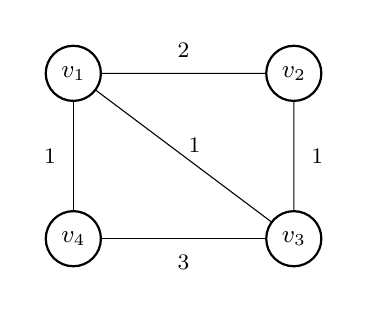
\begin{tikzpicture}[scale=1.4,
    every node/.style={circle, draw, minimum size=0.7cm, font=\small, thick}]
    \node (1) at (0,1.5) {$v_1$};
    \node (2) at (2,1.5) {$v_2$};
    \node (3) at (2,0) {$v_3$};
    \node (4) at (0,0) {$v_4$};
    \draw (1) -- node[above, draw=none, minimum size=0pt, font=\footnotesize]
      {2} (2);
    \draw (2) -- node[right, draw=none, minimum size=0pt, font=\footnotesize]
      {1} (3);
    \draw (3) -- node[below, draw=none, minimum size=0pt, font=\footnotesize]
      {3} (4);
    \draw (1) -- node[left, draw=none, minimum size=0pt, font=\footnotesize]
      {1} (4);
    \draw (1) -- node[above right=-2pt, draw=none, minimum size=0pt,
      font=\footnotesize] {1} (3);
\end{tikzpicture}
\end{center}

\[
A = \begin{pmatrix} 0&2&1&1 \\ 2&0&1&0 \\ 1&1&0&3 \\ 1&0&3&0 \end{pmatrix}, \quad
D = \diag(4,3,5,4)
\]
This graph is \textbf{not regular}: $d_2 = 3 \neq 5 = d_3$.
\end{numericalexample}

\subsection{Graph Laplacian Matrices}

The Laplacian is the most important matrix in spectral graph theory. To
motivate it, consider this question: given a function $f: V \to \R$ that
assigns a real number to each node (e.g., a class score or a temperature),
\emph{how can we measure how much $f$ varies across the graph?} A natural
answer is to sum the squared differences along edges:
$\sum_{\{i,j\} \in E} A_{ij}(f_i - f_j)^2$. The Laplacian is the matrix that
computes this sum via a simple quadratic form.

\begin{definition}[Unnormalized (Combinatorial) Laplacian]
\label{semi-supervised-graphs:def:laplacian}
$L = D - A$.
\end{definition}

The following theorem makes precise the connection between $L$ and the
``edge variation'' of a signal:

\begin{theorem}[Laplacian Quadratic Form]
\label{semi-supervised-graphs:thm:laplacian_quadratic}
Let $G$ be an undirected graph (i.e., $A = A^\top$, $A_{ij} \geq 0$).
For any $f \in \R^n$:
\begin{equation}
\label{semi-supervised-graphs:eq:quad_form}
f^\top L f = \frac{1}{2}\sum_{i=1}^n \sum_{j=1}^n A_{ij}(f_i - f_j)^2
\end{equation}
\end{theorem}

\begin{proof}
$f^\top L f = f^\top D f - f^\top A f = \sum_i d_i f_i^2 - \sum_{i,j} A_{ij}f_if_j
= \sum_{i,j} A_{ij}f_i^2 - \sum_{i,j} A_{ij}f_if_j$.

Since $A_{ij} = A_{ji}$ (undirected), $\sum_{i,j} A_{ij}f_i^2
= \frac{1}{2}\bigl(\sum_{i,j} A_{ij}f_i^2 + \sum_{i,j} A_{ji}f_j^2\bigr)
= \frac{1}{2}\sum_{i,j} A_{ij}(f_i^2 + f_j^2)$.

Similarly $\sum_{i,j} A_{ij}f_if_j = \frac{1}{2}\sum_{i,j}A_{ij}\cdot 2f_if_j$.
Subtracting:
$f^\top L f = \frac{1}{2}\sum_{i,j}A_{ij}(f_i^2 - 2f_if_j + f_j^2)
= \frac{1}{2}\sum_{i,j}A_{ij}(f_i - f_j)^2$.
\end{proof}

\begin{warningbox}
\textbf{Undirectedness is essential.} The proof uses $A_{ij} = A_{ji}$ to
symmetrize. For a directed graph, $L = D_{\mathrm{out}} - A$ is non-symmetric,
$f^\top Lf$ need not equal~\eqref{semi-supervised-graphs:eq:quad_form}, and $L$ need not be positive
semi-definite.
\end{warningbox}

\begin{numericalexample}[title=Verifying the Quadratic Form]
From example~\ref{semi-supervised-graphs:numex:4node} with $f = (1,2,0,-1)^\top$:
\[
L = D - A = \begin{pmatrix}
4&{-2}&{-1}&{-1}\\{-2}&3&{-1}&0\\{-1}&{-1}&5&{-3}\\{-1}&0&{-3}&4
\end{pmatrix}
\]

\textbf{Direct:} $f^\top Lf = 1(1) + 2(4) + 0(0) + (-1)(-5) = 14$.

\textbf{Edge sum} (each undirected edge $\{i,j\}$ contributes
$A_{ij}(f_i - f_j)^2$):
$2(1{-}2)^2 + 1(1{-}0)^2 + 1(1{-}(-1))^2 + 1(2{-}0)^2 + 3(0{-}(-1))^2
= 2+1+4+4+3 = 14$ \checkmark
\end{numericalexample}

\begin{proposition}[Properties of the Unnormalized Laplacian]
\label{semi-supervised-graphs:prop:laplacian_properties}
For a connected undirected graph $G$ with $n$ nodes:
\begin{enumerate}
    \item $L$ is symmetric ($L = L^\top$) and positive semi-definite
      ($f^\top Lf \geq 0$).
    \item Eigenvalues: $0 = \lambda_1 < \lambda_2 \leq \cdots \leq \lambda_n$
      (strict inequality $\lambda_2 > 0$ by connectivity).
    \item $L\mathbf{1} = \mathbf{0}$: the constant vector
      $\mathbf{1} = (1,\ldots,1)^\top$ is the eigenvector for $\lambda_1 = 0$.
    \item $\lambda_2$ is called the \emph{algebraic connectivity}
      (Fiedler value); it measures how well-connected $G$ is.
\end{enumerate}
\end{proposition}

\begin{proof}
(1) Symmetry: $L^\top = (D-A)^\top = D^\top - A^\top = D - A = L$.
PSD: by Theorem~\ref{semi-supervised-graphs:thm:laplacian_quadratic},
$f^\top Lf = \frac{1}{2}\sum_{ij}A_{ij}(f_i - f_j)^2 \geq 0$.

(2--3) $L\mathbf{1} = D\mathbf{1} - A\mathbf{1} = (d_1,\ldots,d_n)^\top
- (d_1,\ldots,d_n)^\top = \mathbf{0}$, so $\lambda_1 = 0$.

(4) If $\lambda_2 = 0$, there exists $f \perp \mathbf{1}$ with
$f^\top Lf = 0$, i.e., $f_i = f_j$ whenever $A_{ij} > 0$. By connectivity,
$f$ is constant on all of $V$, so $f \propto \mathbf{1}$, contradicting
$f \perp \mathbf{1}$ and $f \neq \mathbf{0}$. Hence $\lambda_2 > 0$.
\end{proof}

\begin{definition}[Normalized Laplacians]
\label{semi-supervised-graphs:def:normalized_laplacians}
The unnormalized Laplacian $L$ treats all nodes equally, but in many
applications high-degree nodes (hubs) dominate the quadratic form $f^\top Lf$
simply because they have more edges. To account for this, we normalize by node
degrees. Two normalizations arise naturally:

\textbf{Symmetric normalization} produces the \textbf{normalized adjacency}
$S$ and the corresponding Laplacian:
\begin{equation}
S = D^{-1/2}AD^{-1/2}, \qquad
\mathcal{L}_{\mathrm{sym}} = I - S = D^{-1/2}LD^{-1/2}
\end{equation}
Here $S_{ij} = A_{ij}/\sqrt{d_id_j}$: the edge weight is divided
symmetrically between both endpoints. $S$ is symmetric, which is convenient
for spectral analysis. $S$ is used in \textbf{label spreading}
(Section~\ref{semi-supervised-graphs:subsec:ls}), \textbf{correct \& smooth} (Section~\ref{semi-supervised-graphs:sec:cs}),
and \textbf{GCN} (Section~\ref{semi-supervised-graphs:sec:gnn}).

\textbf{Random-walk normalization} produces the \textbf{transition matrix}
$P$ and the corresponding Laplacian:
\begin{equation}
P = D^{-1}A, \qquad \mathcal{L}_{\mathrm{rw}} = I - P = D^{-1}L
\end{equation}
Here $P_{ij} = A_{ij}/d_i$: the weight is divided by the degree of the
\emph{source} node only, making each row sum to 1 (a probability distribution).
$P$ defines a random walk (Section~\ref{semi-supervised-graphs:subsec:random_walks}) and is used in
\textbf{label propagation} (Section~\ref{semi-supervised-graphs:subsec:lp_algo}).
\end{definition}

\begin{proposition}[Properties of $S$, $P$, and the Normalized Laplacians]
\label{semi-supervised-graphs:prop:normalized_properties}
For a connected undirected graph:
\begin{enumerate}
    \item $S$ is symmetric; $P$ is generally \textbf{not} symmetric (unless
      $G$ is regular).
    \item $P$ is \textbf{row-stochastic}: $\sum_j P_{ij} = 1$ for all $i$
      (each row is a probability distribution).
    \item $S$ is \textbf{not} row-stochastic in general
      (see Remark~\ref{semi-supervised-graphs:rem:row_sums}).
    \item $S$ and $P$ have the same eigenvalues (they are similar:
      $P = D^{-1/2}SD^{1/2}$).
    \item Eigenvalues of $S$ lie in $[-1, 1]$, with $1$ being the largest
      eigenvalue.
    \item $\mathcal{L}_{\mathrm{sym}}$ has eigenvalues in $[0, 2]$;
      $\mathcal{L}_{\mathrm{sym}}$ and $\mathcal{L}_{\mathrm{rw}}$ share
      eigenvalues.
\end{enumerate}
\end{proposition}

\begin{proof}
(1) $S^\top = (D^{-1/2}AD^{-1/2})^\top = D^{-1/2}A^\top D^{-1/2} = S$.
For $P$: $(D^{-1}A)^\top = A^\top D^{-1} = AD^{-1} \neq D^{-1}A$ unless
$D \propto I$ (regular).

(2) $\sum_j P_{ij} = \sum_j A_{ij}/d_i = d_i/d_i = 1$.

(3) See Remark~\ref{semi-supervised-graphs:rem:row_sums}.

(4) $P = D^{-1}A = D^{-1/2}(D^{-1/2}AD^{-1/2})D^{1/2}
= D^{-1/2}SD^{1/2}$. Similar matrices share eigenvalues.

(5) Since $L$ is PSD (Proposition~\ref{semi-supervised-graphs:prop:laplacian_properties}) and
$D^{-1/2}$ is invertible, the congruence $\mathcal{L}_{\mathrm{sym}}
= D^{-1/2}LD^{-1/2}$ is PSD (for any invertible $M$ and PSD matrix $B$,
$M^\top BM \succeq 0$). Hence $I - S = \mathcal{L}_{\mathrm{sym}} \succeq 0$.

\emph{Upper bound $\sigma_k \leq 1$.} Let $v_k$ be a unit eigenvector of $S$
with eigenvalue $\sigma_k$. Because $I - S \succeq 0$:
\[
  0 \;\leq\; v_k^\top(I - S)v_k \;=\; \|v_k\|^2 - \sigma_k\|v_k\|^2
  \;=\; 1 - \sigma_k,
\]
so $\sigma_k \leq 1$.

\emph{Lower bound $\sigma_k \geq -1$.} Similarly, $I + S
= 2I - \mathcal{L}_{\mathrm{sym}}$ is PSD~\cite{semi-supervised-graphs:chung1997}
(it equals $D^{-1/2}(2D - L)D^{-1/2} = D^{-1/2}(D+A)D^{-1/2}$, which is PSD
since $D + A \succeq 0$ entry-wise). Applying the same argument to $I + S$
gives $1 + \sigma_k \geq 0$, i.e.\ $\sigma_k \geq -1$.

\emph{The eigenvalue $1$ is attained.} The vector $D^{1/2}\mathbf{1}$ is an
eigenvector for eigenvalue $1$:
\[
  S\bigl(D^{1/2}\mathbf{1}\bigr)
  = D^{-1/2}AD^{-1/2}D^{1/2}\mathbf{1}
  = D^{-1/2}A\mathbf{1}
  = D^{-1/2}D\mathbf{1}
  = D^{1/2}\mathbf{1}. \qedhere
\]
\end{proof}

\begin{remark}[Row Sums of $S$]
\label{semi-supervised-graphs:rem:row_sums}
A common error is claiming $\sum_j S_{ij} = 1$. In fact:
$\sum_j S_{ij} = \sum_j \frac{A_{ij}}{\sqrt{d_i}\sqrt{d_j}}
= \frac{1}{\sqrt{d_i}}\sum_j \frac{A_{ij}}{\sqrt{d_j}}$.
This equals $1$ iff all neighbors $j$ of $i$ have degree $d_j = d_i$---i.e.,
only for regular graphs (Definition~\ref{semi-supervised-graphs:def:regular}).
\end{remark}

\begin{numericalexample}[title=Comparing $P$ and $S$]
From the 4-node graph ($D = \diag(4,3,5,4)$):

$P = D^{-1}A$: row 1 = $(0,\; 1/2,\; 1/4,\; 1/4)$, sum $= 1$ \checkmark\;
(row-stochastic).

$S_{12} = \frac{2}{\sqrt{4}\sqrt{3}} = \frac{1}{\sqrt{3}} \approx 0.577$, \;
$S_{13} = \frac{1}{\sqrt{4}\sqrt{5}} = \frac{1}{2\sqrt{5}} \approx 0.224$, \;
$S_{14} = \frac{1}{\sqrt{4}\sqrt{4}} = \frac{1}{4}$.

Row 1 sum of $S$: $0 + 0.577 + 0.224 + 0.250 = 1.051 \neq 1$ \;
($S$ is \textbf{not} row-stochastic).
\end{numericalexample}

\subsection{Random Walks on Graphs}
\label{semi-supervised-graphs:subsec:random_walks}

The transition matrix $P = D^{-1}A$ has a natural probabilistic interpretation
that provides deep intuition for label propagation.

\begin{definition}[Random Walk]
A \textbf{random walk} on $G$ is a sequence of nodes $(X_0, X_1, X_2, \ldots)$
where at each step, the walker moves from its current node to a random
neighbor, with probability proportional to the edge weight:
if $X_t = v_i$, then $\Pr(X_{t+1} = v_j) = P_{ij} = A_{ij}/d_i$.
\end{definition}

\begin{insightbox}
\textbf{Random walks and label propagation.}
Consider an unlabeled node $v_i$. Start a random walk at $v_i$ and let it
wander until it first hits a labeled node. The probability that this walk hits
labeled node $v_j$ (before any other labeled node) turns out to be exactly
$Y_i^*[j]$---the label propagation solution. In other words, label propagation
computes \emph{absorption probabilities} of random walks.

This interpretation explains several features of the algorithm. (i) The
iterative form $Y^{(t)} = PY^{(t-1)}$ simulates one walk step per iteration.
(ii) Clamping ensures that once a walk reaches a labeled node, it ``absorbs''
there. (iii) Nodes far from all labeled nodes converge slowly because walks
take many steps to reach them.
\end{insightbox}

\subsection{Reproducing Kernel Hilbert Spaces (RKHS)}
\label{semi-supervised-graphs:subsec:rkhs}

In Section~\ref{semi-supervised-graphs:sec:reg}, we will want to combine graph smoothness with a
classical machine learning model (like an SVM). The challenge is: how do we
optimize over a rich, possibly infinite-dimensional class of functions while
keeping the problem tractable? The RKHS framework provides the answer. The key
result---the Representer Theorem---guarantees that even when we search over
infinitely many functions, the optimal solution always has a finite,
computable form. We develop this theory here.

\begin{definition}[Positive Definite Kernel]
\label{semi-supervised-graphs:def:kernel}
A function $K: \mathcal{X} \times \mathcal{X} \to \R$ is a
\textbf{positive definite (p.d.) kernel} if it is symmetric
($K(x, x') = K(x', x)$) and for any $m \geq 1$, any $x_1, \ldots, x_m
\in \mathcal{X}$, and any $c_1, \ldots, c_m \in \R$:
\begin{equation}
\sum_{i=1}^m \sum_{j=1}^m c_i c_j K(x_i, x_j) \geq 0
\end{equation}
Common examples: the Gaussian (RBF) kernel
$K(x,x') = \exp(-\|x - x'\|^2 / 2\sigma^2)$ and the polynomial kernel
$K(x,x') = (\inner{x}{x'} + c)^p$.
\end{definition}

\begin{definition}[Kernel (Gram) Matrix]
\label{semi-supervised-graphs:def:gram}
Given data points $x_1, \ldots, x_n$ and kernel $K$, the \textbf{kernel matrix}
(or \textbf{Gram matrix}) is $\mathbf{K} \in \R^{n \times n}$ with entries
$\mathbf{K}_{ij} = K(x_i, x_j)$. By the p.d.\ property, $\mathbf{K}$ is
symmetric and positive semi-definite. This is a concrete, computable
$n \times n$ matrix---it will play a central role below.
\end{definition}

\begin{definition}[Reproducing Kernel Hilbert Space]
\label{semi-supervised-graphs:def:rkhs}
Given a p.d.\ kernel $K$, the \textbf{RKHS} $\mathcal{H}_K$ is the unique
Hilbert space of functions $f: \mathcal{X} \to \R$ satisfying:
\begin{enumerate}
    \item \textbf{Feature map}: For each $x \in \mathcal{X}$, the function
      $K(\cdot, x)$ belongs to $\mathcal{H}_K$.
    \item \textbf{Reproducing property}:
      $f(x) = \inner{f}{K(\cdot, x)}_{\mathcal{H}_K}$ for all
      $f \in \mathcal{H}_K$.
\end{enumerate}
The RKHS norm $\|f\|_{\mathcal{H}_K}$ measures the ``complexity'' of $f$;
smoother functions have smaller norm.
\end{definition}

\begin{theorem}[Representer Theorem~\cite{semi-supervised-graphs:scholkopf2001}]
\label{semi-supervised-graphs:thm:representer}
Consider any optimization problem of the form
\begin{equation}
\label{semi-supervised-graphs:eq:representer_problem}
\min_{f \in \mathcal{H}_K}\; \sum_{i=1}^n \ell(f(x_i), y_i) + 
\lambda \|f\|_{\mathcal{H}_K}^2
\end{equation}
where $\ell$ is any loss function and $\lambda > 0$. Then the minimizer has
the finite expansion:
\begin{equation}
\label{semi-supervised-graphs:eq:representer_solution}
f^*(x) = \sum_{i=1}^n \alpha_i K(x, x_i) \quad
\text{for some } \alpha_1, \ldots, \alpha_n \in \R
\end{equation}
\end{theorem}

The proof is given in Appendix~\ref{semi-supervised-graphs:app:representer}.

\begin{remark}[We never need to know $\mathcal{H}_K$ explicitly---the
  ``kernel trick'']
\label{semi-supervised-graphs:rem:rkhs_practical}
The search ``$\min_{f \in \mathcal{H}_K}$'' over an infinite-dimensional space
may seem hopeless: we cannot enumerate or even concretely describe
$\mathcal{H}_K$. The Representer Theorem resolves this: the minimizer always
lies in $\mathrm{span}\{K(\cdot, x_1), \ldots, K(\cdot, x_n)\}$, so the
problem reduces to finding $n$ real numbers $\alpha_1, \ldots, \alpha_n$.

Let us make this concrete. Substituting~\eqref{semi-supervised-graphs:eq:representer_solution} into
~\eqref{semi-supervised-graphs:eq:representer_problem}:

\textbf{Loss term:} $f^*(x_i) = \sum_{j=1}^n \alpha_j K(x_i, x_j)
= (\mathbf{K}\boldsymbol{\alpha})_i$ where $\mathbf{K}$ is the Gram matrix
(Definition~\ref{semi-supervised-graphs:def:gram}) and $\boldsymbol{\alpha}
= (\alpha_1, \ldots, \alpha_n)^\top$.

\textbf{Regularizer:} $\|f^*\|_{\mathcal{H}_K}^2
= \sum_{i,j}\alpha_i\alpha_j K(x_i, x_j)
= \boldsymbol{\alpha}^\top \mathbf{K}\,\boldsymbol{\alpha}$
(derived in Appendix~\ref{semi-supervised-graphs:app:representer}).

Together, the infinite-dimensional problem~\eqref{semi-supervised-graphs:eq:representer_problem}
becomes:
\begin{equation}
\label{semi-supervised-graphs:eq:kernelized_problem}
\min_{\boldsymbol{\alpha} \in \R^n}\;
\sum_{i=1}^n \ell\!\left((\mathbf{K}\boldsymbol{\alpha})_i,\; y_i\right) +
\lambda\, \boldsymbol{\alpha}^\top \mathbf{K}\, \boldsymbol{\alpha}
\end{equation}
This is a standard finite-dimensional optimization over
$\boldsymbol{\alpha} \in \R^n$, involving only the computable Gram matrix
$\mathbf{K}$.
\end{remark}

\subsection{The Spectral Radius}
\label{semi-supervised-graphs:subsec:spectral_radius}

Every iterative algorithm in this document (label propagation, label spreading,
correct \& smooth) converges because a certain matrix has spectral radius less
than 1. We define this concept here so it is ready when we need it.

\begin{definition}[Spectral Radius]
\label{semi-supervised-graphs:def:spectral_radius}
Let $M \in \R^{n \times n}$. A scalar $\lambda \in \mathbb{C}$ is an
\textbf{eigenvalue} of $M$ if there exists a nonzero vector $v$ with
$Mv = \lambda v$. The \textbf{spectral radius} of $M$ is the largest
eigenvalue magnitude:
\begin{equation}
\rho(M) = \max\{|\lambda| : \lambda \text{ is an eigenvalue of } M\}
\end{equation}
\end{definition}

The spectral radius tells us whether repeatedly multiplying by $M$ amplifies
or dampens:

\begin{proposition}[Powers and the Spectral Radius]
\label{semi-supervised-graphs:prop:spectral_powers}
$M^t \to 0$ as $t \to \infty$ if and only if $\rho(M) < 1$.
\end{proposition}

\begin{proof}
See Appendix~\ref{semi-supervised-graphs:app:spectral_radius}.
\end{proof}

\begin{numericalexample}[title=Spectral Radius]
For $M = \begin{psmallmatrix} 0 & 1/2 \\ 1/2 & 0 \end{psmallmatrix}$,
eigenvalues are $\pm 1/2$, so $\rho(M) = 1/2 < 1$. Indeed:
$M^2 = \frac{1}{4}I$, $M^4 = \frac{1}{16}I$, $M^t \to 0$.

For $M = \begin{psmallmatrix} 0 & 1 \\ 1 & 0 \end{psmallmatrix}$,
eigenvalues are $\pm 1$, so $\rho(M) = 1$, and $M^t$ oscillates without
converging to 0.
\end{numericalexample}

\subsection{Label Matrix and Partitioning}

\begin{definition}[Label Matrix]
\label{semi-supervised-graphs:def:label_matrix}
For $C$-class classification, the \textbf{label matrix} $Y \in \R^{n \times C}$
encodes class assignments: $Y_{ic} = 1$ if node $v_i$ has label $c$, and
$Y_{ic} = 0$ otherwise. For labeled nodes, row $Y_i$ is a one-hot vector;
for unlabeled nodes, $Y_i = \mathbf{0}^\top$ (all zeros).
\end{definition}

\begin{definition}[Block Partitioning]
\label{semi-supervised-graphs:def:partitioning}
Reorder nodes so that the $l$ labeled nodes come first, followed by the $u$
unlabeled nodes ($l + u = n$). This induces a $2\times 2$ block structure on
every $n \times n$ matrix:
\[
Y = \begin{pmatrix} Y_L \\ Y_U \end{pmatrix}, \quad
A = \begin{pmatrix} A_{LL} & A_{LU} \\ A_{UL} & A_{UU} \end{pmatrix}, \quad
P = \begin{pmatrix} P_{LL} & P_{LU} \\ P_{UL} & P_{UU} \end{pmatrix}
\]
where $Y_L \in \R^{l \times C}$ contains the known labels,
$Y_U \in \R^{u \times C}$ is initially zero,
$A_{LU} \in \R^{l \times u}$ encodes edges \emph{between} labeled and
unlabeled nodes, etc.
\end{definition}

\begin{numericalexample}[title=Label Matrix and Partitioning on a 6-Node Graph]
Consider a graph with 6 nodes, 2 classes (Red $=1$, Green $=2$), and 2 labeled
nodes ($v_1$: Red, $v_2$: Green):

\begin{center}
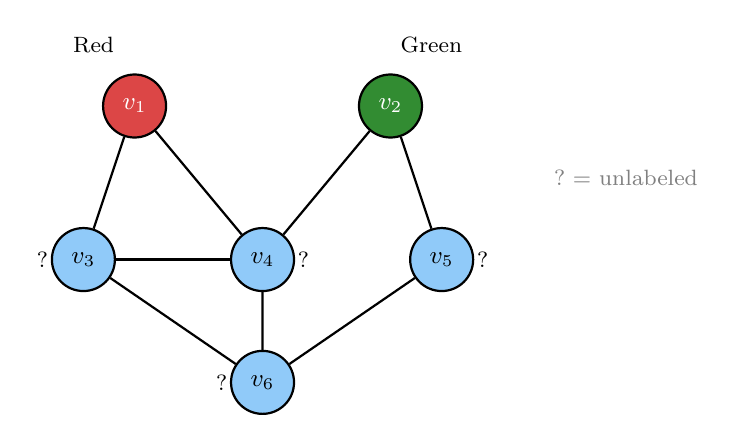
\begin{tikzpicture}[scale=1.3,
    labeled/.style={circle, draw, thick, minimum size=0.8cm, font=\small\bfseries,
      text=white},
    unlabeled/.style={circle, draw, thick, minimum size=0.8cm, font=\small,
      fill=unlabeledblue}]
    
    % Nodes
    \node[labeled, fill=labeledred] (1) at (0, 1.5) {$v_1$};
    \node[labeled, fill=labeledgreen] (2) at (2.5, 1.5) {$v_2$};
    \node[unlabeled] (3) at (-0.5, 0) {$v_3$};
    \node[unlabeled] (4) at (1.25, 0) {$v_4$};
    \node[unlabeled] (5) at (3, 0) {$v_5$};
    \node[unlabeled] (6) at (1.25, -1.2) {$v_6$};
    
    % Edges
    \draw[thick] (1) -- (3);
    \draw[thick] (1) -- (4);
    \draw[thick] (2) -- (4);
    \draw[thick] (2) -- (5);
    \draw[thick] (3) -- (4);
    \draw[thick] (3) -- (6);
    \draw[thick] (4) -- (6);
    \draw[thick] (5) -- (6);
    
    % Legend
    \node[draw=none, font=\footnotesize] at (-0.4, 2.1) {Red};
    \node[draw=none, font=\footnotesize] at (2.9, 2.1) {Green};
    \node[draw=none, font=\footnotesize] at (-0.9, 0) {?};
    \node[draw=none, font=\footnotesize] at (1.65, 0) {?};
    \node[draw=none, font=\footnotesize] at (3.4, 0) {?};
    \node[draw=none, font=\footnotesize] at (0.85, -1.2) {?};
    \node[draw=none, font=\footnotesize, text=gray] at (4.8, 0.8)
      {$?$ = unlabeled};
\end{tikzpicture}
\end{center}

\textbf{Labeled set:} $\mathcal{V}_L = \{v_1, v_2\}$ (nodes come first after
reordering). \textbf{Unlabeled set:} $\mathcal{V}_U = \{v_3, v_4, v_5, v_6\}$.

\textbf{Label matrix} ($C = 2$ classes):
\[
Y = \begin{pmatrix} Y_L \\ \hline Y_U \end{pmatrix}
= \left(\begin{array}{cc} 1 & 0 \\ 0 & 1 \\ \hline 0 & 0 \\ 0 & 0 \\
0 & 0 \\ 0 & 0 \end{array}\right)
\quad \leftarrow \begin{array}{l} v_1 \text{ is Red} \\ v_2 \text{ is Green} \\
v_3 \text{ unknown} \\ v_4 \text{ unknown} \\ v_5 \text{ unknown} \\
v_6 \text{ unknown} \end{array}
\]

\textbf{Adjacency matrix} (unweighted, so $A_{ij} \in \{0,1\}$), partitioned:
\[
A = \left(\begin{array}{cc|cccc}
0 & 0 & 1 & 1 & 0 & 0 \\
0 & 0 & 0 & 1 & 1 & 0 \\
\hline
1 & 0 & 0 & 1 & 0 & 1 \\
1 & 1 & 1 & 0 & 0 & 1 \\
0 & 1 & 0 & 0 & 0 & 1 \\
0 & 0 & 1 & 1 & 1 & 0
\end{array}\right)
= \begin{pmatrix} A_{LL} & A_{LU} \\ A_{UL} & A_{UU} \end{pmatrix}
\]

Reading the blocks: $A_{LU} = \bigl(\begin{smallmatrix} 1&1&0&0 \\ 0&1&1&0
\end{smallmatrix}\bigr)$ encodes which unlabeled nodes are neighbors of each
labeled node (e.g., $v_1$ connects to $v_3, v_4$). $A_{UU}$ encodes edges
among unlabeled nodes only.

\textbf{Transition matrix} $P = D^{-1}A$ with $D = \diag(2, 2, 3, 4, 2, 3)$:
\[
P_{UL} = \begin{pmatrix} 1/3 & 0 \\ 1/4 & 1/4 \\ 0 & 1/2 \\ 0 & 0 \end{pmatrix},
\quad
P_{UU} = \begin{pmatrix} 0 & 1/3 & 0 & 1/3 \\ 1/4 & 0 & 0 & 1/4 \\
0 & 0 & 0 & 1/2 \\ 1/3 & 1/3 & 1/3 & 0 \end{pmatrix}
\]

\textbf{Interpretation:} $P_{UL}$ tells us how much ``label information'' each
unlabeled node receives directly from labeled nodes. For instance, $v_4$ gets
$1/4$ of its weight from $v_1$ (Red) and $1/4$ from $v_2$ (Green). Node $v_6$
has $P_{v_6, L} = (0, 0)$: it receives \emph{no direct label information}---
it can only be classified through multi-hop propagation via $P_{UU}$.
\end{numericalexample}


\newpage
\section{Label Propagation Algorithms}
\label{semi-supervised-graphs:sec:lp}

We now turn to the central question of this document: given a graph with a
few labeled nodes and many unlabeled ones, how do we predict the labels of the
unlabeled nodes using only the graph structure (no node features)?

The core idea is remarkably intuitive: \emph{let each node adopt the
consensus of its neighbors}. If we repeat this averaging process---while
keeping the labeled nodes fixed---the label information gradually diffuses
through the graph until every node has a prediction. This is
\textbf{label propagation}.

\begin{insightbox}
\textbf{Diffusion analogy.} Think of the graph as a network of pipes
connecting containers of water. Labeled nodes are faucets held at fixed
temperatures: class $A =$ ``hot,'' class $B =$ ``cold.'' At each time step,
every container equilibrates with its neighbors. Over time, the temperature
field reaches a smooth interpolation---hot near class~$A$ sources, cold near
class~$B$, and tepid in between. Label propagation formalizes this process
using the transition matrix $P = D^{-1}A$ from
Section~\ref{semi-supervised-graphs:subsec:random_walks}.
\end{insightbox}

\subsection{Label Propagation (Zhu \& Ghahramani, 2002)}
\label{semi-supervised-graphs:subsec:lp_algo}

\begin{algorithm}[H]
\caption{Label Propagation~\cite{semi-supervised-graphs:zhu2002}}
\label{semi-supervised-graphs:alg:label_prop}
\begin{algorithmic}[1]
\State \textbf{Input:} Graph $G$, labeled set $\mathcal{V}_L$, labels $Y_L$,
        max iterations $T$, tolerance $\epsilon$
\State \textbf{Initialize:} $Y_U^{(0)} = \mathbf{0}$
\State Compute $P = D^{-1}A$
\For{$t = 1, 2, \ldots, T$}
    \State $Y^{(t)} = P \, Y^{(t-1)}$
      \Comment{Diffuse: each node averages its neighbors}
    \State $Y_L^{(t)} = Y_L$ \Comment{Clamp: reset labeled nodes}
    \If{$\|Y^{(t)} - Y^{(t-1)}\|_F < \epsilon$} \textbf{break} \EndIf
\EndFor
\State \textbf{Output:} $\hat{y}_i = \argmax_c Y_{ic}^{(T)}$ for
      $i \in \mathcal{V}_U$
\end{algorithmic}
\end{algorithm}

The algorithm alternates two operations. \textbf{Diffuse} (step~5): every
node---labeled and unlabeled---replaces its current label distribution by the
weighted average of its neighbors' distributions. This is simply
multiplication by the transition matrix $P$. \textbf{Clamp} (step~6): the
labeled nodes are reset to their known labels, undoing any change the
diffusion made to them.

Why is clamping necessary? Without it, the original labels would be diluted
and eventually lost---every node would converge to the same global average.
Clamping ensures that labeled nodes act as permanent ``anchors'' that
continually inject label information into the graph.

In the block-partitioned form (Definition~\ref{semi-supervised-graphs:def:partitioning}), clamping
means the update for unlabeled nodes is:
\begin{equation}
\label{semi-supervised-graphs:eq:lp_update}
Y_U^{(t)} = P_{UL}\,Y_L + P_{UU}\,Y_U^{(t-1)}
\end{equation}
The first term $P_{UL}Y_L$ is the direct contribution from labeled neighbors
(constant across iterations, thanks to clamping). The second term
$P_{UU}Y_U^{(t-1)}$ is the contribution from other unlabeled neighbors,
which evolves over time.

\subsection{Convergence and Closed-Form Solution}

Does the iteration~\eqref{semi-supervised-graphs:eq:lp_update} converge? If so, to what?

\begin{theorem}[Closed-Form Solution and Convergence]
\label{semi-supervised-graphs:thm:lp_closed}
Let $G$ be a connected graph (Standing Assumption~\ref{semi-supervised-graphs:def:standing}) with at
least one labeled node. Then label propagation converges to
$Y_U^* = (I - P_{UU})^{-1}P_{UL}Y_L$.
\end{theorem}

\begin{warningbox}
\textbf{Connectivity is essential.} This is the first place in the document
where connectivity is genuinely used. If $G$ is disconnected, consider an
unlabeled node $v_i$ in a connected component that contains \emph{no} labeled
nodes. Every neighbor of $v_i$ is also unlabeled, so
$\sum_{j \in \mathcal{V}_U}(P_{UU})_{ij} = \sum_j P_{ij} = 1$: no
probability leaks to labeled nodes. On such a component, $P_{UU}$ is
(fully) stochastic, $\rho(P_{UU}) = 1$, and the iteration does not converge.
In practice, if a graph has multiple connected components, label propagation
must be applied to each component separately, and any component without
labeled nodes cannot be classified by this method.
\end{warningbox}

\begin{proof}
We proceed in three steps, carefully ordering existence before convergence.
\vspace{0.5em}

\textbf{Step 1: $\rho(P_{UU}) < 1$ and existence of $Y_U^*$.}
Since $P$ is row-stochastic ($\sum_j P_{ij} = 1$), the submatrix $P_{UU}$ has
row sums:
\[
\sum_{j \in \mathcal{V}_U} (P_{UU})_{ij}
= 1 - \underbrace{\sum_{j \in \mathcal{V}_L} P_{ij}}_{=:\,\ell_i} \;\leq\; 1,
\]
where $\ell_i \geq 0$ is the \textbf{one-step escape probability} at $v_i$:
the probability that a random walker at $v_i$ jumps directly into
$\mathcal{V}_L$ in one step. Since $G$ is connected and has at least one
labeled node, every unlabeled node $v_i$ adjacent to a labeled node satisfies
$\ell_i > 0$, giving a strictly sub-unit row sum. A non-negative matrix whose
row sums are all $\leq 1$ with at least one strictly $< 1$ is called
\textbf{sub-stochastic}. We show in Appendix~\ref{semi-supervised-graphs:app:substochastic} that
sub-stochasticity together with connectivity implies $\rho(P_{UU}) < 1$.

Since $\rho(P_{UU}) < 1$, the matrix $I - P_{UU}$ is invertible
(all its eigenvalues $1 - \sigma_k$ satisfy $|1-\sigma_k| \geq 1 - \rho(P_{UU})
> 0$). We therefore \emph{define}:
\[
  Y_U^* \;:=\; (I - P_{UU})^{-1}\,P_{UL}\,Y_L.
\]

\textbf{Step 2: $Y_U^*$ is a fixed point of the iteration.}
We verify by direct substitution that $Y_U^*$ satisfies the
update~\eqref{semi-supervised-graphs:eq:lp_update}:
\[
  P_{UL}Y_L + P_{UU}Y_U^*
  = P_{UL}Y_L + P_{UU}(I-P_{UU})^{-1}P_{UL}Y_L
  = \bigl(I + P_{UU}(I-P_{UU})^{-1}\bigr)P_{UL}Y_L.
\]
Using the identity $I + P_{UU}(I-P_{UU})^{-1} = (I-P_{UU})^{-1}$
(multiply both sides on the right by $(I-P_{UU})$ to verify), we get:
\[
  P_{UL}Y_L + P_{UU}Y_U^* = (I-P_{UU})^{-1}P_{UL}Y_L = Y_U^*.
\]
So $Y_U^*$ is indeed a fixed point. No circularity: we derived the fixed-point
equation from the explicit formula, not the other way around.

\textbf{Step 3: The iteration converges to $Y_U^*$.}
Now that $Y_U^*$ exists and is verified to be a fixed point, define the error
$e^{(t)} := Y_U^{(t)} - Y_U^*$. Using~\eqref{semi-supervised-graphs:eq:lp_update} and the fixed-point
equation from Step~2:
\begin{align}
e^{(t)} &= Y_U^{(t)} - Y_U^* \notag\\
&= \bigl(P_{UL}Y_L + P_{UU}Y_U^{(t-1)}\bigr)
 - \bigl(P_{UL}Y_L + P_{UU}Y_U^*\bigr) \notag\\
&= P_{UU}\bigl(Y_U^{(t-1)} - Y_U^*\bigr) = P_{UU}\,e^{(t-1)}.
\end{align}
The $P_{UL}Y_L$ terms cancel because clamping keeps the labeled contribution
identical at every step. Applying the recurrence:
$e^{(t)} = P_{UU}^t\,e^{(0)}$.
Since $\rho(P_{UU}) < 1$, Proposition~\ref{semi-supervised-graphs:prop:spectral_powers} gives
$P_{UU}^t \to 0$, hence $e^{(t)} \to 0$ and $Y_U^{(t)} \to Y_U^*$.
\end{proof}

\begin{remark}[Why use the iterative form in practice?]
\label{semi-supervised-graphs:rem:why_iterative}
The closed-form $Y_U^* = (I - P_{UU})^{-1}P_{UL}Y_L$ is elegant but
requires inverting a $u \times u$ matrix ($O(u^3)$ operations). For
$u = 10^6$ unlabeled nodes, this is intractable. By contrast, each iteration
of~\eqref{semi-supervised-graphs:eq:lp_update} costs only $O(|E| \cdot C)$---one sparse
matrix-vector product per class---and convergence typically takes 10--50
iterations. The iterative form is therefore the practical choice for large
graphs.
\end{remark}

\subsection{The Harmonic Property}
\label{semi-supervised-graphs:subsec:harmonic}

The closed-form solution has an elegant mathematical characterization that
connects label propagation to a classical topic in mathematics:
\emph{harmonic functions} and \emph{boundary value problems}. This
perspective reveals that label propagation is not just a clever heuristic---it
is the unique solution to a well-posed mathematical problem.

\subsubsection*{What does ``harmonic'' mean on a graph?}

In everyday language, a function is ``harmonic'' at a point if its value there
equals the average of its values nearby. On a graph, ``nearby'' means
``neighbors'':

\begin{definition}[Harmonic Function on a Graph]
\label{semi-supervised-graphs:def:harmonic}
A function $f: V \to \R$ is \textbf{harmonic at node $v_i$} if its value
equals the weighted average of $f$ over the neighbors of $v_i$:
\begin{equation}
\label{semi-supervised-graphs:eq:harmonic_condition}
f(v_i) = \sum_{j \in \mathcal{N}(i)} \frac{A_{ij}}{d_i}\,f(v_j)
= \sum_j P_{ij}\,f(v_j)
\end{equation}
A function is \textbf{harmonic on a set $S \subset V$} if it is harmonic at
every node in $S$.
\end{definition}

In other words, a harmonic function has \emph{no local extrema} on the
interior: no node can have a value strictly larger (or smaller) than all its
neighbors. Its value is always a compromise between its neighbors' values.
This is exactly what the diffusion process in label propagation produces---the
iteration keeps averaging until every unlabeled node is at the ``consensus''
of its neighborhood.

\subsubsection*{Connection to classical mathematics}

The word ``harmonic'' comes from the theory of vibrations and heat, where
harmonic functions describe equilibrium states. In continuous mathematics,
a function $f : \R^d \to \R$ is harmonic if its Laplacian vanishes:
$\Delta f = \sum_k \frac{\partial^2 f}{\partial x_k^2} = 0$. Such functions
satisfy the \textbf{mean value property}: the value of $f$ at any point
equals the average of $f$ over any sphere centered at that point. Harmonic
functions arise whenever a system reaches equilibrium---steady-state
temperature distributions, electric potentials, and fluid pressures are all
harmonic.

On a graph, the random-walk Laplacian gives the discrete version:
\begin{equation}
(\mathcal{L}_{\mathrm{rw}} f)_i = f_i - \sum_j P_{ij}\,f_j
\end{equation}
Setting $(\mathcal{L}_{\mathrm{rw}} f)_i = 0$ recovers exactly the harmonic
condition~\eqref{semi-supervised-graphs:eq:harmonic_condition}. So ``harmonic on a graph'' and
``in the null space of the graph Laplacian (restricted to interior nodes)''
are the same thing.

\subsubsection*{The boundary value problem}

In many physical problems, we know the value of a quantity on the boundary of
a region and want to find its values in the interior. For example: we know
the temperature on the walls of a room and want to find the steady-state
temperature at every point inside. This is a \emph{Dirichlet boundary value
problem}.

\begin{definition}[Dirichlet Boundary Value Problem on a Graph]
\label{semi-supervised-graphs:def:dirichlet}
Given a graph $G$, a set of \textbf{boundary nodes} $\mathcal{V}_L$ with
prescribed values $f(v_i) = y_i$ for $i \in \mathcal{V}_L$, find a function
$f : V \to \R$ that is \textbf{harmonic on the interior}
$\mathcal{V}_U = V \setminus \mathcal{V}_L$ while respecting the boundary
values.
\end{definition}

The parallel to semi-supervised learning is immediate: the boundary
nodes are the labeled nodes, the boundary values are the labels, and the
interior is the set of unlabeled nodes whose values we seek. Label
propagation is literally solving a boundary value problem on the graph.

\subsubsection*{Label propagation solves the Dirichlet problem}

\begin{proposition}[Harmonic Property of Label Propagation]
\label{semi-supervised-graphs:prop:harmonic}
The label propagation solution $Y_U^*$ is harmonic on $\mathcal{V}_U$ with
Dirichlet boundary conditions $Y_L$. That is, label propagation solves the
discrete Dirichlet boundary value problem.
\end{proposition}

\begin{proof}
The proof is immediate from the fixed-point equation. At convergence, for
each unlabeled node $i \in \mathcal{V}_U$:
\[
Y_i^* = \sum_j P_{ij}\,Y_j^*
\]
This is precisely the harmonic condition
(Definition~\ref{semi-supervised-graphs:def:harmonic}). Meanwhile, the clamping step ensures
$Y_j^* = y_j$ for all $j \in \mathcal{V}_L$ (the Dirichlet boundary
condition).
\end{proof}

\subsubsection*{Worked example: verifying harmonicity}

To make this concrete, consider a small weighted triangle where we can check
every condition by hand.

\begin{figure}[ht]
\centering
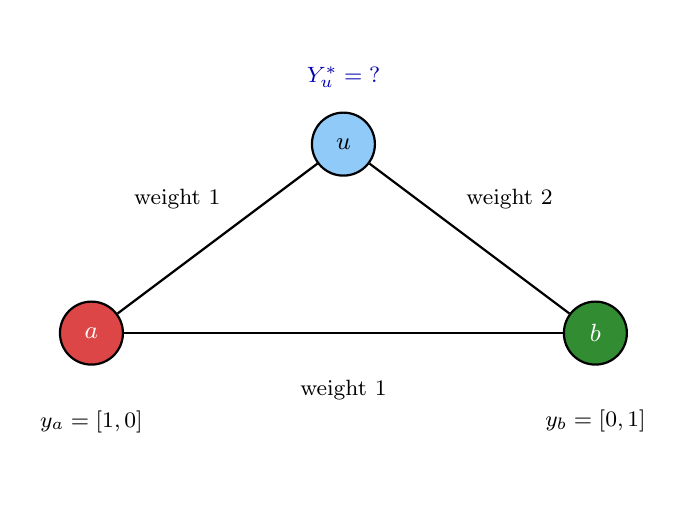
\begin{tikzpicture}[scale=1.6,
    every node/.style={circle, draw, minimum size=0.8cm, font=\small, thick}]
    \node[fill=labeledred, text=white, font=\small\bfseries] (A) at (0,0) {$a$};
    \node[fill=labeledgreen, text=white, font=\small\bfseries] (B) at (4,0) {$b$};
    \node[fill=unlabeledblue] (U) at (2,1.5) {$u$};
    
    \draw[thick] (A) -- node[below, draw=none, minimum size=0pt,
      font=\footnotesize] {weight 1} (B);
    \draw[thick] (A) -- node[above left, draw=none, minimum size=0pt,
      font=\footnotesize] {weight 1} (U);
    \draw[thick] (B) -- node[above right, draw=none, minimum size=0pt,
      font=\footnotesize] {weight 2} (U);
    
    \node[below=0.3cm, draw=none, font=\footnotesize] at (A)
      {$y_a = [1,0]$};
    \node[below=0.3cm, draw=none, font=\footnotesize] at (B)
      {$y_b = [0,1]$};
    \node[above=0.2cm, draw=none, font=\footnotesize, text=blue!70!black]
      at (U) {$Y_u^* = \;?$};
\end{tikzpicture}
\caption{Triangle graph with two labeled boundary nodes ($a$, $b$) and one
  unlabeled interior node ($u$). Edge weights are shown. The harmonic solution
  at $u$ must equal the weighted average of its neighbors' values.}
\label{semi-supervised-graphs:fig:harmonic_triangle}
\end{figure}

Node $u$ has degree $d_u = 1 + 2 = 3$ (sum of incident edge weights), so the
transition probabilities from $u$ are $P_{ua} = 1/3$ and $P_{ub} = 2/3$.
The harmonic condition (Definition~\ref{semi-supervised-graphs:def:harmonic}) requires:
\[
Y_u^* = P_{ua}\,y_a + P_{ub}\,y_b
= \tfrac{1}{3}\,[1,0] + \tfrac{2}{3}\,[0,1] = [\,1/3,\; 2/3\,]
\]
Node $u$ is predicted as class $B$ (Green) with probability $2/3$---reflecting
the fact that its edge to $b$ is twice as strong as its edge to $a$. The
stronger connection ``pulls'' $u$ toward $b$'s label, just as a heavier pipe
carries more heat from a heat source.

This is the unique harmonic function on $\{u\}$ with boundary values
$y_a = [1,0]$ and $y_b = [0,1]$. No other assignment to $u$ satisfies the
averaging property.

\begin{insightbox}
\textbf{Resistor network interpretation.} The connection between harmonic
functions and electrical circuits is classical. Each edge with weight $A_{ij}$
acts as a conductor with conductance $A_{ij}$ (resistance $1/A_{ij}$). The
labeled nodes are connected to batteries at fixed voltages (class
$A = 1\text{V}$, class $B = 0\text{V}$). By Kirchhoff's current law, the
current flowing into any interior node must equal the current flowing out;
this balance condition is precisely the harmonic
equation~\eqref{semi-supervised-graphs:eq:harmonic_condition}. Label propagation computes the
equilibrium voltages.

In the triangle above, node $u$ is connected to the $1$V source (node $a$)
by a conductor of conductance~$1$ and to the $0$V source (node $b$) by a
conductor of conductance~$2$. More current flows from $b$ (higher
conductance), pulling $u$'s voltage toward $0$V. The result,
$V_u = 1/3 \approx 0.33\text{V}$, is consistent with $Y_u^*[A] = 1/3$.
\end{insightbox}

\subsection{Numerical Example}
\label{semi-supervised-graphs:subsec:lp_example}

\begin{example}[Label Propagation on a Path Graph]
\label{semi-supervised-graphs:ex:lp_path}
Consider the simplest interesting case: a path graph with five nodes, where
only the two endpoints are labeled.

\begin{center}
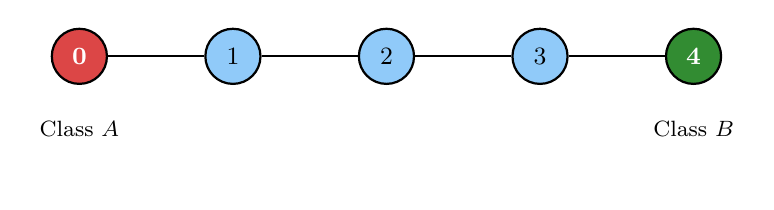
\begin{tikzpicture}[scale=1.5,
    every node/.style={circle, draw, minimum size=0.7cm, font=\small, thick}]
    \node[fill=labeledred, text=white, font=\small\bfseries] (0) at (0,0) {0};
    \node[fill=unlabeledblue] (1) at (1.3,0) {1};
    \node[fill=unlabeledblue] (2) at (2.6,0) {2};
    \node[fill=unlabeledblue] (3) at (3.9,0) {3};
    \node[fill=labeledgreen, text=white, font=\small\bfseries] (4) at (5.2,0) {4};
    \draw[thick] (0)--(1)--(2)--(3)--(4);
    \node[below=0.25cm, draw=none, font=\footnotesize] at (0) {Class $A$};
    \node[below=0.25cm, draw=none, font=\footnotesize] at (4) {Class $B$};
\end{tikzpicture}
\end{center}

The interior nodes $1, 2, 3$ are unlabeled. Since each interior node has
exactly two neighbors, the transition matrix gives equal weight $1/2$ to each:

$P_{UU} = \begin{psmallmatrix} 0 & 1/2 & 0 \\ 1/2 & 0 & 1/2 \\
0 & 1/2 & 0 \end{psmallmatrix}$, \;
$P_{UL} = \begin{psmallmatrix} 1/2 & 0 \\ 0 & 0 \\ 0 & 1/2 \end{psmallmatrix}$.

\noindent Note that $P_{UU}$ is sub-stochastic: the rows of nodes 1 and 3 sum
to $1/2$ (they each have a labeled neighbor), while node~2's row sums to~1
(both neighbors are unlabeled). Nonetheless, since node~2 can reach a labeled
node in two steps, the walk eventually escapes, and $\rho(P_{UU}) < 1$.

Solving $(I - P_{UU})Y_U^* = P_{UL}I_2$:

\[
(I - P_{UU})^{-1} = \begin{pmatrix}
3/2 & 1 & 1/2 \\ 1 & 2 & 1 \\ 1/2 & 1 & 3/2
\end{pmatrix} \implies
Y_U^* = \begin{pmatrix} 3/4 & 1/4 \\ 1/2 & 1/2 \\ 1/4 & 3/4 \end{pmatrix}
\]

\begin{center}
\begin{tabular}{c|cc|c}
\toprule Node & $P(A)$ & $P(B)$ & Prediction \\ \midrule
0 & 1.00 & 0.00 & $A$ (given) \\
1 & 0.75 & 0.25 & $A$ \\
2 & 0.50 & 0.50 & Tie \\
3 & 0.25 & 0.75 & $B$ \\
4 & 0.00 & 1.00 & $B$ (given) \\ \bottomrule
\end{tabular}
\end{center}

The result is a linear interpolation between the two boundary labels---exactly
what the diffusion analogy predicts. We can verify the harmonic property at
node~2: $Y_2^* = \frac{1}{2}Y_1^* + \frac{1}{2}Y_3^*
= \frac{1}{2}(3/4,1/4) + \frac{1}{2}(1/4,3/4) = (1/2,1/2)$ \checkmark.

The random walk interpretation (Section~\ref{semi-supervised-graphs:subsec:random_walks}) also
applies: a walk starting at node~1 reaches node~0 (class $A$) before node~4
(class $B$) with probability $3/4$.
\end{example}

\subsection{Label Spreading (Zhou et al., 2004)}
\label{semi-supervised-graphs:subsec:ls}

Label propagation's hard clamping means that if a labeled node has an
\emph{incorrect} label (noise), this error propagates permanently through the
graph. Label spreading~\cite{semi-supervised-graphs:zhou2004} introduces \textbf{soft clamping}:
labeled nodes can be updated by the diffusion, but a ``spring'' force pulls
them back toward their initial values:

\begin{algorithm}[H]
\caption{Label Spreading~\cite{semi-supervised-graphs:zhou2004}}
\begin{algorithmic}[1]
\State \textbf{Input:} Graph $G$, initial labels $Y^{(0)}$, parameter
      $\alpha \in (0,1)$, tolerance $\epsilon$
\State Compute $S = D^{-1/2}AD^{-1/2}$
\For{$t = 1, 2, \ldots$}
    \State $Y^{(t)} = \alpha\, S\, Y^{(t-1)} + (1-\alpha)\, Y^{(0)}$
    \If{$\|Y^{(t)} - Y^{(t-1)}\|_F < \epsilon$} \textbf{break} \EndIf
\EndFor
\State \textbf{Output:} $\hat{y}_i = \argmax_c Y_{ic}^{(T)}$
\end{algorithmic}
\end{algorithm}

\noindent \textbf{Key differences from label propagation:}
\begin{itemize}
    \item Uses $S = D^{-1/2}AD^{-1/2}$ (symmetric, degree-normalized)
    instead of $P = D^{-1}A$ (row-stochastic)
    \item Even labeled nodes are updated; the term $(1{-}\alpha)Y^{(0)}$
    pulls them back toward initial values. Parameter $\alpha \to 1$:
    trust graph more; $\alpha \to 0$: trust labels more
\end{itemize}

\begin{theorem}[Label Spreading: Closed Form and Convergence]
\label{semi-supervised-graphs:thm:ls_closed}
Label spreading converges to $Y^* = (1-\alpha)(I - \alpha S)^{-1}Y^{(0)}$, and
the inverse exists for all $\alpha \in (0,1)$.
\end{theorem}

\begin{proof}
We follow the same logical order as in Theorem~\ref{semi-supervised-graphs:thm:lp_closed}: first
establish existence of $Y^*$ by direct construction, then verify it is a fixed
point, then prove the iteration converges to it.
\vspace{0.5em}

\textbf{Step 1: Invertibility of $I - \alpha S$ and existence of $Y^*$.}
By Proposition~\ref{semi-supervised-graphs:prop:normalized_properties}(5), the eigenvalues $\sigma_k$
of $S$ satisfy $\sigma_k \in [-1, 1]$. Hence the eigenvalues of $\alpha S$ lie
in $[-\alpha, \alpha]$, and those of $I - \alpha S$ lie in
$[1-\alpha,\, 1+\alpha] \subset (0, 2)$ for any $\alpha \in (0,1)$. Since all
eigenvalues are strictly positive, $I - \alpha S$ is positive definite, hence
invertible. We therefore \emph{define}:
\[
  Y^* \;:=\; (1-\alpha)(I - \alpha S)^{-1}\,Y^{(0)}.
\]

\textbf{Step 2: $Y^*$ is a fixed point of the iteration.}
We verify by direct substitution that $Y^*$ satisfies the update
$Y = \alpha S Y + (1-\alpha)Y^{(0)}$:
\[
  \alpha S Y^* + (1-\alpha)Y^{(0)}
  = \alpha S\,(1-\alpha)(I-\alpha S)^{-1}Y^{(0)} + (1-\alpha)Y^{(0)}
  = (1-\alpha)\bigl(\alpha S(I-\alpha S)^{-1} + I\bigr)Y^{(0)}.
\]
Using the identity $I + \alpha S(I - \alpha S)^{-1} = (I - \alpha S)^{-1}$
(multiply both sides on the right by $(I - \alpha S)$ to verify), we get:
\[
  \alpha S Y^* + (1-\alpha)Y^{(0)}
  = (1-\alpha)(I - \alpha S)^{-1}Y^{(0)} = Y^*.
\]
So $Y^*$ is indeed a fixed point, derived from its explicit formula without
any circularity.

\textbf{Step 3: The iteration converges to $Y^*$.}
Now that $Y^*$ exists and is a fixed point, define $e^{(t)} := Y^{(t)} - Y^*$.
Using the update rule and the fixed-point equation from Step~2:
\begin{align}
e^{(t)} &= Y^{(t)} - Y^* \notag\\
&= \bigl(\alpha S Y^{(t-1)} + (1-\alpha)Y^{(0)}\bigr)
 - \bigl(\alpha S Y^* + (1-\alpha)Y^{(0)}\bigr) \notag\\
&= \alpha S\bigl(Y^{(t-1)} - Y^*\bigr) = \alpha S\,e^{(t-1)}.
\end{align}
The $(1-\alpha)Y^{(0)}$ terms cancel identically at every step. Applying the
recurrence: $e^{(t)} = (\alpha S)^t\,e^{(0)}$. Since $\rho(\alpha S) \leq
\alpha < 1$, Proposition~\ref{semi-supervised-graphs:prop:spectral_powers} gives $(\alpha S)^t \to 0$,
hence $e^{(t)} \to 0$ and $Y^{(t)} \to Y^*$.
\end{proof}

\begin{theorem}[Variational Formulation]
\label{semi-supervised-graphs:thm:ls_energy}
Label spreading minimizes a well-defined energy function that balances two
competing objectives:
\begin{equation}
\mathcal{E}(F) = 
\underbrace{\sum_{\{i,j\}\in E} A_{ij}\left(\frac{F_i}{\sqrt{d_i}} -
\frac{F_j}{\sqrt{d_j}}\right)^2}_{\mathclap{\substack{
    \text{normalized smoothness:}\\ 
    \text{``nearby nodes should agree''}}}} \; + \; \frac{1-\alpha}{\alpha}\,
\underbrace{\sum_{i=1}^n \|F_i - Y_i^{(0)}\|^2}_{\mathclap{\substack{
    \text{label fitting:}\\
    \text{``don't stray from initial labels''}}}}
\end{equation}
\end{theorem}

This variational perspective is important for two reasons. First, it shows
that label spreading is not merely an ad-hoc iterative scheme---it is solving
a principled optimization problem with a clear objective. Second, the two
terms reveal the tradeoff controlled by $\alpha$: when $\alpha$ is large, the
smoothness term dominates and the solution follows the graph structure; when
$\alpha$ is small, the fitting term dominates and the solution stays close to
the initial labels.

\begin{proof}
See Appendix~\ref{semi-supervised-graphs:app:ls_energy}.
\end{proof}

\section{Correct and Smooth}
\label{semi-supervised-graphs:sec:cs}

Label propagation and label spreading operate directly on the label matrix
$Y$. But what if we already have a powerful base predictor (e.g., a neural
network trained on node features) that produces soft predictions
$\hat{Y} \in \R^{n \times C}$? Can we use the graph to \emph{correct} and
\emph{smooth} these predictions without retraining?

Correct and Smooth (C\&S)~\cite{semi-supervised-graphs:huang2021} answers this question with a
surprisingly simple and effective two-stage post-processing method. It has
become a standard component in many graph learning pipelines, often providing
substantial improvements at near-zero additional cost.

\begin{insightbox}
\textbf{Core idea:} Base model predictions contain systematic errors that are
\emph{correlated along graph edges}. If node $v$ misclassifies, its neighbors
likely make similar mistakes. We can estimate these errors from labeled nodes
and propagate them to correct unlabeled nodes. Then we smooth the corrected
predictions to enforce local consistency.
\end{insightbox}

\subsection{Intuition: Errors Are Contagious}

Consider a simple binary classification problem on a graph with high homophily.
A base model (e.g., a multilayer perceptron trained only on node features)
produces predictions $\hat{y}_i \in [0,1]$ for each node. On labeled nodes, we
can compute the \textbf{training error}:
\begin{equation}
E_i = y_i - \hat{y}_i \quad \text{for } i \in \mathcal{V}_L
\end{equation}

These errors are not random noise---they reflect systematic biases in the base
model. Crucially, due to homophily, if the base model under-predicts the
probability of class $A$ for a labeled node, it likely under-predicts for that
node's neighbors as well. Therefore, we can \textbf{propagate} these errors
from labeled to unlabeled nodes to correct their predictions.

\subsection{Stage 1: Correcting Predictions}

Let $\hat{Y} \in \R^{n \times C}$ be the base model's soft predictions
(typically logits or probabilities). Define the \textbf{error matrix}
$E \in \R^{n \times C}$ where:
\begin{equation}
E_{i} = \begin{cases}
Y_i - \hat{Y}_i & \text{if } i \in \mathcal{V}_L \\
\mathbf{0} & \text{if } i \in \mathcal{V}_U
\end{cases}
\end{equation}

We now propagate these errors using $k$ steps of label propagation with the
normalized adjacency $S = D^{-1/2}AD^{-1/2}$:

\begin{correctionbox}
\textbf{Error propagation:}
\begin{equation}
E^{(0)} = E, \quad E^{(t+1)} = (1-\alpha) E + \alpha S E^{(t)}
\end{equation}
or equivalently in closed form:
\begin{equation}
E^* = (1-\alpha)(I - \alpha S)^{-1} E
\end{equation}

The corrected predictions are:
\begin{equation}
\hat{Y}^{\text{corr}} = \hat{Y} + E^*
\end{equation}
\end{correctionbox}

The hyperparameter $\alpha \in (0,1)$ controls how much error information flows
from labeled nodes. Higher $\alpha$ means longer-range propagation. In practice,
$k$ is often set to a small integer (e.g., 5--10) rather than iterating to
convergence.

\begin{remark}[Why propagate errors, not labels?]
Directly propagating labels (as in label propagation) ignores the base model's
predictions entirely. C\&S preserves the base model's output and only corrects
its \emph{residuals}. This is analogous to boosting: we fit a model to the
errors of a base learner.
\end{remark}

\subsection{Stage 2: Smoothing Predictions}

After correction, the predictions $\hat{Y}^{\text{corr}}$ may still be noisy
and not locally consistent. The smoothing stage applies another round of
diffusion, this time on the corrected predictions themselves:

\begin{smoothingbox}
\textbf{Prediction smoothing:}
\begin{equation}
Z^{(0)} = \hat{Y}^{\text{corr}}, \quad Z^{(t+1)} = (1-\beta) \hat{Y}^{\text{corr}} + \beta S Z^{(t)}
\end{equation}
or in closed form:
\begin{equation}
Z^* = (1-\beta)(I - \beta S)^{-1} \hat{Y}^{\text{corr}}
\end{equation}
\end{smoothingbox}

Why smooth after correcting? The correction step adds a propagated error signal
that may be noisy, especially for nodes far from labeled examples. Smoothing
enforces that neighboring nodes have similar predictions, leveraging the graph
homophily assumption.

\begin{warningbox}
\textbf{Critical:} Smoothing uses $\hat{Y}^{\text{corr}}$ as the ``base''
predictions, not $\hat{Y}$. The term $(1-\beta)\hat{Y}^{\text{corr}}$ in each
iteration pulls the smoothed predictions back toward the \emph{corrected} values,
not the original noisy predictions. This prevents the smoothing step from
undoing the correction.
\end{warningbox}

\subsection{Mathematical Justification}

C\&S can be understood as solving two separate graph-regularized optimization
problems, each of the same form as label spreading
(Theorem~\ref{semi-supervised-graphs:thm:ls_energy}). This variational perspective reveals \emph{why}
the two-stage pipeline is principled: both stages are not ad-hoc diffusion
steps, but optimal solutions to well-posed smoothness problems.

\subsubsection*{The common structure}

Both stages minimize an objective of the form
\begin{equation}
\label{semi-supervised-graphs:eq:cs_general_opt}
\min_{F \in \R^{n \times C}}\;
\underbrace{\|F - B\|_F^2}_{\text{stay close to }B}
\;+\; \mu \underbrace{\sum_{i,j}A_{ij}
\left\|\frac{F_i}{\sqrt{d_i}} - \frac{F_j}{\sqrt{d_j}}\right\|^2}_{
\mathclap{\substack{{=\,2\,\tr(F^\top \mathcal{L}_{\mathrm{sym}} F)}\\
\text{(normalized smoothness)}}}}
\end{equation}
for a ``target'' matrix $B$ and trade-off parameter $\mu > 0$.
The closed-form solution to~\eqref{semi-supervised-graphs:eq:cs_general_opt} is
$(I + 2\mu\,\mathcal{L}_{\mathrm{sym}})^{-1}B$,
which can be rewritten in the label-spreading form
$(1-\alpha)(I - \alpha S)^{-1}B$ by choosing $\alpha = 1/(1+2\mu)$
(see Appendix~\ref{semi-supervised-graphs:app:cs_opt}). The two stages of C\&S correspond to two
instances of this template with different choices of $B$.

\begin{theorem}[Correct Step as Optimization]
\label{semi-supervised-graphs:thm:cs_correct_opt}
The error propagation $E^* = (1-\alpha)(I - \alpha S)^{-1}E$ is the unique
minimizer of:
\begin{equation}
\min_{F \in \R^{n \times C}}\; \|F - E\|_F^2
  + \frac{\alpha}{1-\alpha}\sum_{i,j}A_{ij}
  \left\|\frac{F_i}{\sqrt{d_i}} - \frac{F_j}{\sqrt{d_j}}\right\|^2
\end{equation}
That is, $E^*$ is the smoothest signal (in the normalized-Laplacian sense) that
remains close to the observed error matrix $E$. Since $E$ is nonzero only on
labeled nodes, the optimization spreads these errors to unlabeled nodes via the
graph structure.
\end{theorem}

\begin{theorem}[Smooth Step as Optimization]
\label{semi-supervised-graphs:thm:cs_smooth_opt}
The smoothed predictions $Z^* = (1-\beta)(I - \beta S)^{-1}\hat{Y}^{\text{corr}}$
are the unique minimizer of:
\begin{equation}
\min_{F \in \R^{n \times C}}\; \|F - \hat{Y}^{\text{corr}}\|_F^2
  + \frac{\beta}{1-\beta}\sum_{i,j}A_{ij}
  \left\|\frac{F_i}{\sqrt{d_i}} - \frac{F_j}{\sqrt{d_j}}\right\|^2
\end{equation}
That is, $Z^*$ is the smoothest signal that stays close to the corrected
predictions $\hat{Y}^{\text{corr}}$.
\end{theorem}

Both theorems are proved in Appendix~\ref{semi-supervised-graphs:app:cs_opt}. The proofs follow the
same template as the label spreading energy proof
(Appendix~\ref{semi-supervised-graphs:app:ls_energy}): compute the gradient, show it vanishes at the
claimed solution, and verify the Hessian is positive definite.

\begin{insightbox}
\textbf{What the variational view adds.} Beyond formal justification, the
variational formulation clarifies the role of $\alpha$ and $\beta$: they are
not arbitrary damping parameters but control the trade-off between fidelity to
the input ($\|F - B\|_F^2$) and graph smoothness. A large $\alpha$ (close to
1) makes the smoothness term cheap relative to fidelity, allowing the error
signal to spread far across the graph; a small $\alpha$ confines corrections to
nodes near labeled examples. The two stages are therefore interpretable as
independent regularized least-squares problems with a shared graph prior.
\end{insightbox}

\subsection{Numerical Example}
\begin{figure}[ht]
\centering
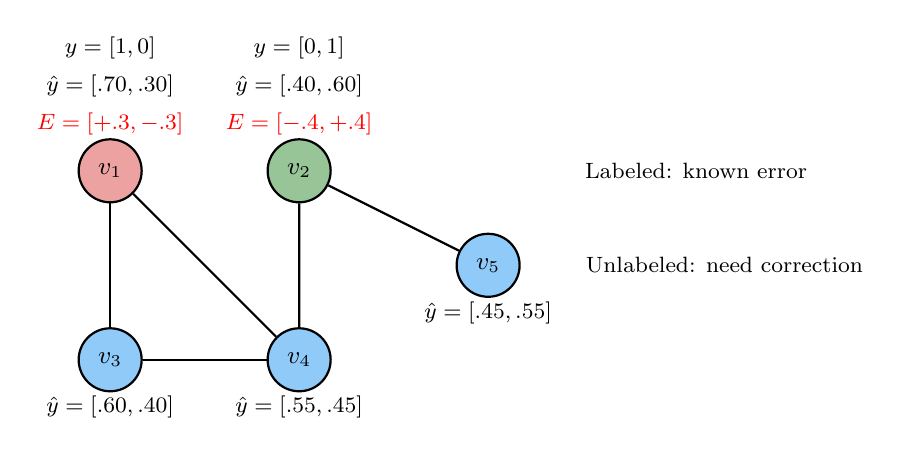
\begin{tikzpicture}[scale=1.2,
    node/.style={circle, draw, thick, minimum size=0.8cm, font=\small}]
    
    % Graph structure
    \node[node, fill=labeledred!50] (1) at (0,2) {$v_1$};
    \node[node, fill=labeledgreen!50] (2) at (2,2) {$v_2$};
    \node[node, fill=unlabeledblue] (3) at (0,0) {$v_3$};
    \node[node, fill=unlabeledblue] (4) at (2,0) {$v_4$};
    \node[node, fill=unlabeledblue] (5) at (4,1) {$v_5$};
    
    \draw[thick] (1) -- (3);
    \draw[thick] (1) -- (4);
    \draw[thick] (2) -- (4);
    \draw[thick] (2) -- (5);
    \draw[thick] (3) -- (4);
    
    % Labels and predictions
    \node[draw=none, font=\footnotesize] at (0,3.3) {$y=[1,0]$};
    \node[draw=none, font=\footnotesize] at (0,2.9) {$\hat{y}=[.70,.30]$};
    \node[draw=none, font=\footnotesize] at (2,3.3) {$y=[0,1]$};
    \node[draw=none, font=\footnotesize] at (2,2.9) {$\hat{y}=[.40,.60]$};
    \node[draw=none, font=\footnotesize] at (0,-0.5) {$\hat{y}=[.60,.40]$};
    \node[draw=none, font=\footnotesize] at (2,-0.5) {$\hat{y}=[.55,.45]$};
    \node[draw=none, font=\footnotesize] at (4,0.5) {$\hat{y}=[.45,.55]$};
    
    % Errors
    \node[draw=none, font=\footnotesize, text=red] at (0,2.5) {$E=[+.3,-.3]$};
    \node[draw=none, font=\footnotesize, text=red] at (2,2.5) {$E=[-.4,+.4]$};
    
    % Legend
    \node[draw=none, font=\footnotesize] at (6.2,2) {Labeled: known error};
    \node[draw=none, font=\footnotesize] at (6.5,1) {Unlabeled: need correction};
\end{tikzpicture}
\caption{C\&S setup. Degrees: $d_1 = d_2 = d_3 = 2$, $d_4 = 3$, $d_5 = 1$.}
\label{semi-supervised-graphs:fig:cs_error}
\end{figure}

Consider the 5-node graph from Figure~\ref{semi-supervised-graphs:fig:cs_error}. A base model
trained on node features produces predictions $\hat{Y}$ (shown). We apply
C\&S with $\alpha = \beta = 0.7$.
\vspace{0.5em}

\textbf{Step 1: Correct.} The error matrix $E$ is nonzero only on labeled
nodes: $E_1 = [+0.3, -0.3]$ (base model under-predicts Red for $v_1$),
$E_2 = [-0.4, +0.4]$ (under-predicts Green for $v_2$). Error propagation
via $E^{(t+1)} = 0.3\,E + 0.7\,S\,E^{(t)}$ spreads these errors through
the graph. To understand how, consider the first iteration. The product
$S\,E$ gives the error that each unlabeled node receives from its neighbors:
\begin{itemize}
    \item $v_3$ (neighbors: $v_1, v_4$) receives $[+0.15, -0.15]$---mainly
          from $v_1$'s positive Red error. Since $v_4$ has no error yet,
          only $v_1$ contributes.
    \item $v_4$ (neighbors: $v_1, v_2, v_3$) receives $[{-0.04}, {+0.04}]$.
          This small value arises because $v_1$'s error
          $S_{41}\!\cdot\![+0.3,-0.3] = [+0.12, -0.12]$ and $v_2$'s error
          $S_{42}\!\cdot\![-0.4,+0.4] = [-0.16, +0.16]$ \textbf{partially
          cancel}. Node $v_4$ sits between the two labeled nodes, so the
          opposing corrections nearly neutralize.
    \item $v_5$ (neighbor: $v_2$ only) receives $[-0.28, +0.28]$---a strong
          correction toward Green, because $v_5$ is connected only to $v_2$.
\end{itemize}
After convergence, the propagated errors $E^*$ are added to $\hat{Y}$
and labeled nodes are clamped to their true labels.
\vspace{0.5em}

\textbf{Step 2: Smooth.} Smoothing via
$Z^{(t+1)} = 0.3\,\hat{Y}^{\text{corr}} + 0.7\,S\,Z^{(t)}$ averages
each node's prediction with its neighbors' corrected predictions:
\begin{itemize}
    \item $v_1$ (neighbors: $v_3, v_4$): pulled from $[1.00, 0.00]$
          (clamped) toward the average of $v_3$ and $v_4$'s corrected
          predictions $([0.63 + 0.54]/2 \approx 0.59$), yielding
          $[0.72, 0.28]$. Still Red, but the extreme clamped value is
          softened.
    \item $v_2$ (neighbors: $v_4, v_5$): pulled from $[0.00, 1.00]$
          (clamped) toward $v_4$ and $v_5$'s corrected values, yielding
          $[0.30, 0.70]$.
    \item $v_3$ (neighbors: $v_1, v_4$): its corrected prediction
          $[0.63, 0.37]$ already agrees well with its neighbors
          ($v_1$~is~Red, $v_4$~is~mixed), so smoothing barely changes it:
          $[0.63, 0.37]$.
    \item $v_4$ (neighbors: $v_1, v_2, v_3$): neighbor average is
          $[0.54, 0.46]$, close to $v_4$'s corrected prediction. Smoothing
          leaves it at $[0.54, 0.46]$---balanced between the two classes,
          reflecting its position between the two labeled nodes.
    \item $v_5$ (neighbor: $v_2$ only): pulled further toward Green,
          from $[0.37, 0.63] \to [0.33, 0.67]$. Smoothing reinforces the
          correction.
\end{itemize}

The complete pipeline is summarized in the following table:

\begin{center}
\small
\begin{tabular}{c|c|c|c|c|c|c}
\toprule
Node & True & Base $\hat{Y}$ & Error $E$ & $E^*$ (propagated)
  & Corrected $\hat{Y}^{\text{corr}}$ & Smoothed $Z^*$ \\
\midrule
$v_1$ (R) & [1,0] & [.70,\,.30] & [+.30,$-$.30] & ---
  & [1.00,\,0.00] (clamp) & [\textbf{.72},\,.28] \\
$v_2$ (G) & [0,1] & [.40,\,.60] & [$-$.40,+.40] & ---
  & [0.00,\,1.00] (clamp) & [.30,\,\textbf{.70}] \\
$v_3$ & ? & [.60,\,.40] & [0,\,0] & [+.03,$-$.03]
  & [\textbf{.63},\,.37] & [\textbf{.63},\,.37] \\
$v_4$ & ? & [.55,\,.45] & [0,\,0] & [$-$.01,+.01]
  & [.54,\,.46] & [.54,\,.46] \\
$v_5$ & ? & [.45,\,.55] & [0,\,0] & [$-$.08,+.08]
  & [.37,\,\textbf{.63}] & [.33,\,\textbf{.67}] \\
\bottomrule
\end{tabular}
\end{center}
(Smoothed values are row-normalized. Bold marks the predicted class.)

The key observations: $v_5$'s initial weak lean toward Green ($[0.45, 0.55]$)
has been strengthened to a confident $[0.33, 0.67]$ through both correction and
smoothing. Node $v_4$, sitting between the two labeled nodes, receives almost
no net correction ($E^* \approx 0$) because the opposing errors cancel---and
smoothing confirms this balanced position. Node $v_3$, connected to $v_1$ (Red)
but not $v_2$, is pulled toward Red by both stages.

\subsection{Why C\&S Works So Well}

C\&S achieves state-of-the-art results on many benchmarks with a simple linear
base model. Why?

\begin{enumerate}
    \item \textbf{Decouples feature learning from graph exploitation.}
          The base model learns from features without being distracted by graph
          structure; C\&S then optimally uses the graph to clean up predictions.
    \item \textbf{Avoids over-smoothing.} Unlike GCNs which mix features and
          graph in every layer, C\&S applies only two shallow diffusion steps,
          preventing the node representations from becoming indistinguishable.
    \item \textbf{Computational efficiency.} C\&S requires only sparse matrix
          multiplications and no gradient computation. It scales to graphs with
          billions of edges.
    \item \textbf{Theoretical guarantees.} Under the contextual stochastic
          block model (CSBM), C\&S provably improves the base classifier and
          achieves optimal misclassification rate~\cite{semi-supervised-graphs:huang2021}.
\end{enumerate}

\begin{insightbox}
\textbf{Takeaway:} Before training a complex GNN, try this recipe:
\begin{enumerate}
    \item Train a simple MLP on node features (ignore the graph).
    \item Apply C\&S to the MLP's predictions.
\end{enumerate}
This simple pipeline often outperforms sophisticated GNNs, especially when
features are informative and the graph is moderately homophilic.
\end{insightbox}


\newpage
\section{Graph Regularization Methods}
\label{semi-supervised-graphs:sec:reg}

The label propagation methods of Section~\ref{semi-supervised-graphs:sec:lp} and the post-processing
of Section~\ref{semi-supervised-graphs:sec:cs} use \emph{only} the graph structure to classify nodes
or correct predictions---they either ignore node features entirely or treat
them only through a base model. In many applications (text classification,
molecular property prediction), rich features $x_i \in \R^d$ are available at
each node. How can we combine features with graph structure in a single
end-to-end training objective?

The idea is natural: train a parametric model $f_\theta$ (neural network, SVM,
etc.) on the labeled data as usual, but add a penalty term that discourages
$f_\theta$ from assigning different predictions to connected nodes. This
penalty is the Laplacian quadratic form from Theorem~\ref{semi-supervised-graphs:thm:laplacian_quadratic},
which we already know measures how much a signal varies across edges.

\subsection{General Framework}

\begin{definition}[Graph-Regularized Objective]
\label{semi-supervised-graphs:def:graph_reg}
For a parametric model $f_\theta: \R^d \to \R^C$ mapping node features to
class scores:
\begin{equation}
\label{semi-supervised-graphs:eq:graph_reg}
\mathcal{L}(\theta) = 
\underbrace{
    \sum_{i \in \mathcal{V}_L}\ell(f_\theta(x_i), y_i)}_{
        \mathclap{\substack{\text{supervised loss} \\
        \text{(labeled nodes only)}}}} \; + \;
\lambda\underbrace{\frac{1}{2}\sum_{i,j}A_{ij}\|f_\theta(x_i) - 
f_\theta(x_j)\|^2}_{\mathclap{\substack{\text{graph smoothness} \\
\text{(all nodes, labeled and unlabeled)}}}}
\end{equation}
where $\lambda > 0$ controls the regularization strength.
\end{definition}

The first term is standard supervised learning. The second term involves
\emph{all} nodes (labeled and unlabeled)---this is how unlabeled data enters
the training. Minimizing it pushes the model toward predictions that are smooth
over the graph. We now make precise the connection to the Laplacian.

\begin{remark}[Graph regularizer as a trace form]
\label{semi-supervised-graphs:rem:trace_form}
Define $F \in \R^{n \times C}$ as the matrix whose $i$-th row is
$f_\theta(x_i)^\top \in \R^C$. The graph smoothness term in~\eqref{semi-supervised-graphs:eq:graph_reg}
can be written compactly as:
\begin{equation}
\label{semi-supervised-graphs:eq:trace_form}
\frac{1}{2}\sum_{i=1}^n\sum_{j=1}^n A_{ij}\|f_\theta(x_i) - f_\theta(x_j)\|^2
= \tr(F^\top L F).
\end{equation}
\textbf{Derivation.} Expanding the squared norm class-by-class:
\[
\frac{1}{2}\sum_{i,j}A_{ij}\|F_i - F_j\|^2
= \frac{1}{2}\sum_{i,j}A_{ij}\sum_{c=1}^C(F_{ic}-F_{jc})^2
= \sum_{c=1}^C \frac{1}{2}\sum_{i,j}A_{ij}(F_{ic}-F_{jc})^2.
\]
By Theorem~\ref{semi-supervised-graphs:thm:laplacian_quadratic}, each inner sum equals $f_c^\top L f_c$
where $f_c \in \R^n$ is the $c$-th column of $F$. Summing over $c$:
\[
\sum_{c=1}^C f_c^\top L f_c = \tr(F^\top L F),
\]
since $\tr(F^\top L F) = \sum_c (F^\top L F)_{cc} = \sum_c f_c^\top L f_c$. The
identity~\eqref{semi-supervised-graphs:eq:trace_form} thus follows directly from the scalar quadratic
form of Theorem~\ref{semi-supervised-graphs:thm:laplacian_quadratic}, applied column by column.
\end{remark}

\begin{example}[Symbolic computation of $\tr(F^\top LF)$]
\label{semi-supervised-graphs:ex:trace_form_symbolic}
To make Remark~\ref{semi-supervised-graphs:rem:trace_form} concrete, consider a 3-node path graph
$v_1 - v_2 - v_3$ with unit edge weights ($A_{12} = A_{23} = 1$, all others
zero) and a model with $C = 2$ output classes. The degree matrix and Laplacian
are:
\[
D = \begin{pmatrix} 1 & 0 & 0 \\ 0 & 2 & 0 \\ 0 & 0 & 1 \end{pmatrix}, \qquad
L = D - A = \begin{pmatrix} 1 & -1 & 0 \\ -1 & 2 & -1 \\ 0 & -1 & 1 \end{pmatrix}.
\]
Let the model's output matrix $F \in \R^{3 \times 2}$ be written in terms of
symbolic scores:
\[
F = \begin{pmatrix} a_1 & b_1 \\ a_2 & b_2 \\ a_3 & b_3 \end{pmatrix},
\]
where $F_i = (a_i, b_i)^\top$ is the score vector output by $f_\theta$ at node
$v_i$ (e.g.\ the pre-softmax logits for classes $A$ and $B$).

\textbf{Edge-sum formula.} The two edges of the graph contribute:
\begin{align*}
\frac{1}{2}\sum_{i,j}A_{ij}\|F_i - F_j\|^2
&= A_{12}\|F_1 - F_2\|^2 + A_{23}\|F_2 - F_3\|^2 \\
&= (a_1 - a_2)^2 + (b_1 - b_2)^2
 + (a_2 - a_3)^2 + (b_2 - b_3)^2.
\end{align*}
(Each unordered edge $\{i,j\}$ appears once because the $\frac{1}{2}$ cancels
the double-counting from the double sum, as in Theorem~\ref{semi-supervised-graphs:thm:laplacian_quadratic}.)

\textbf{Trace formula.} We verify that $\tr(F^\top LF)$ gives the same result.
Denote the two columns of $F$ as $f_A = (a_1, a_2, a_3)^\top$ and
$f_B = (b_1, b_2, b_3)^\top$. Then:
\begin{align*}
\tr(F^\top LF) &= f_A^\top L f_A + f_B^\top L f_B.
\end{align*}
Computing $f_A^\top L f_A$ using $L = D - A$:
\begin{align*}
f_A^\top L f_A
&= a_1^2 + 2a_2^2 + a_3^2 - 2a_1 a_2 - 2a_2 a_3 \\
&= (a_1 - a_2)^2 + (a_2 - a_3)^2,
\end{align*}
and analogously $f_B^\top L f_B = (b_1 - b_2)^2 + (b_2 - b_3)^2$. Summing:
\[
\tr(F^\top LF) = (a_1-a_2)^2 + (b_1-b_2)^2 + (a_2-a_3)^2 + (b_2-b_3)^2,
\]
which matches the edge-sum formula exactly.

\textbf{What the penalty encodes.} The regularizer penalizes the model
whenever adjacent nodes receive different scores. The term $(a_1 - a_2)^2$
penalizes disagreement on class $A$ between $v_1$ and $v_2$; similarly for
class $B$ and for the edge $\{v_2, v_3\}$. If the model perfectly respects
the graph structure and assigns identical scores to all three nodes
($a_1 = a_2 = a_3$ and $b_1 = b_2 = b_3$), then $\tr(F^\top LF) = 0$.
The further the scores deviate across edges, the larger the penalty.
\end{example}

\subsection{Manifold Regularization (LapSVM)}
\label{semi-supervised-graphs:subsec:manifold_reg}

\subsubsection*{Setting: scalar-valued functions and binary classification}

The general framework of Definition~\ref{semi-supervised-graphs:def:graph_reg} handles any number of
classes $C$ through the matrix $F \in \R^{n \times C}$ and the trace penalty
$\tr(F^\top LF)$. Manifold regularization~\cite{semi-supervised-graphs:belkin2006} specializes to the
\textbf{binary} ($C = 2$) case and leverages the RKHS framework
(Section~\ref{semi-supervised-graphs:subsec:rkhs}) to search over a rich, possibly infinite-dimensional
class of functions.

In the binary setting, we seek a single \textbf{scalar-valued} function
$f: \mathcal{X} \to \R$. The prediction rule is:
\begin{equation}
\hat{y}_i = \begin{cases} 1 & \text{if } f(x_i) > 0, \\ 0 & \text{if } f(x_i) \leq 0. \end{cases}
\end{equation}
The value $f(x_i) \in \R$ is a \textbf{decision score}, not a probability or a
hard label. Its sign determines the predicted class; its magnitude encodes
confidence---a score far from zero is a high-confidence prediction, while a
score near zero is ambiguous. This is exactly the SVM decision function: the
hypersurface $\{x : f(x) = 0\}$ is the decision boundary, and $|f(x_i)|$ is
the (unnormalized) margin of node $v_i$.

\begin{warningbox}
\textbf{Relationship to the general framework.}
The vector $\mathbf{f} = (f(x_1), \ldots, f(x_n))^\top \in \R^n$ used below
is \emph{not} the same object as the matrix $F \in \R^{n \times C}$ from
Remark~\ref{semi-supervised-graphs:rem:trace_form}. Rather, $\mathbf{f}$ is a single column of $F$,
corresponding to $C = 1$ (or equivalently to one of the two classes in a
one-vs-rest encoding). The scalar quadratic form $\mathbf{f}^\top L\mathbf{f}$
is the special case of $\tr(F^\top LF)$ when $F$ has a single column. For
$C > 2$ classes, manifold regularization generalizes by training $C$ scalar
functions independently (one-vs-rest), with the full penalty recovering
$\tr(F^\top LF)$.
\end{warningbox}

\subsubsection*{The LapSVM objective}

Manifold regularization combines the graph-regularized objective with the RKHS
framework: search for the best \emph{scalar-valued} function in a rich kernel
space $\mathcal{H}_K$, penalizing both RKHS complexity (ambient smoothness in
feature space) and variation along graph edges (intrinsic smoothness on the
data manifold).

\begin{theorem}[Manifold Regularization]
\label{semi-supervised-graphs:thm:manifold_reg}
Consider the problem:
\begin{equation}
\label{semi-supervised-graphs:eq:manifold_reg}
\min_{f \in \mathcal{H}_K}\;
\underbrace{\frac{1}{l}\sum_{i \in \mathcal{V}_L}\ell(f(x_i), y_i)}_{
    \text{supervised loss}} \quad +
\underbrace{\gamma_A\|f\|_{\mathcal{H}_K}^2}_{\substack{\text{ambient
regularizer:}\\\text{smooth in feature space}}} +
\underbrace{\frac{\gamma_I}{n^2}\mathbf{f}^\top L\mathbf{f}}_{\substack{\text{intrinsic
regularizer:}\\\text{smooth along graph edges}}}
\end{equation}
where $f: \mathcal{X} \to \R$ is scalar-valued,
$\mathbf{f} = (f(x_1), \ldots, f(x_n))^\top \in \R^n$ stacks the scalar
decision scores at all $n$ nodes, and $\gamma_A, \gamma_I > 0$.

By the extended Representer Theorem (Appendix~\ref{semi-supervised-graphs:app:manifold}), the minimizer
has the form $f^*(x) = \sum_{i=1}^n \alpha_i K(x, x_i)$, involving
\textbf{all} $n$ data points (not just the $l$ labeled ones).
\end{theorem}

Using the kernelization technique from Remark~\ref{semi-supervised-graphs:rem:rkhs_practical}
(substituting $\mathbf{f} = \mathbf{K}\boldsymbol{\alpha}$ and
$\|f\|_{\mathcal{H}_K}^2 = \boldsymbol{\alpha}^\top\mathbf{K}\boldsymbol{\alpha}$),
the infinite-dimensional problem~\eqref{semi-supervised-graphs:eq:manifold_reg} becomes:
\begin{equation}
\min_{\boldsymbol{\alpha} \in \R^n}\;
\frac{1}{l}\sum_{i \in \mathcal{V}_L}\ell\bigl((\mathbf{K}\boldsymbol{\alpha})_i,\;
y_i\bigr) + \gamma_A\,\boldsymbol{\alpha}^\top\mathbf{K}\boldsymbol{\alpha} +
\frac{\gamma_I}{n^2}\,\boldsymbol{\alpha}^\top\mathbf{K}L\mathbf{K}\boldsymbol{\alpha}
\end{equation}
This is a finite-dimensional optimization over $\boldsymbol{\alpha} \in \R^n$,
solvable by standard methods.

\begin{insightbox}
\textbf{The two regularizers play complementary roles.}

\textbf{Ambient regularizer} $\gamma_A\|f\|_{\mathcal{H}_K}^2$:
Penalizes complexity \emph{in the RKHS} $\mathcal{H}_K$.
For the linear kernel $K(x,x') = x^\top x'$, this reduces to
$\|w\|_2^2$ in $\mathbb{R}^d$ (standard SVM/Ridge regularization).
For nonlinear kernels (RBF, polynomial), it penalizes functions that
are non-smooth with respect to the kernel's feature map.

\textbf{Intrinsic regularizer} $\frac{\gamma_I}{n^2}\mathbf{f}^\top L\mathbf{f}$:
Penalizes the scalar decision function $f$ for varying rapidly
\emph{along graph edges} — equivalently (by Theorem~\ref{semi-supervised-graphs:thm:laplacian_quadratic}),
it penalizes $\sum_{\{i,j\}\in E}A_{ij}(f(x_i)-f(x_j))^2$, the total squared
disagreement across edges. This term involves \emph{all} $n$ nodes---labeled
and unlabeled---which is how unlabeled data shapes the decision boundary.
\end{insightbox}

\subsection{Neural Graph Learning}
\label{semi-supervised-graphs:subsec:neural_graph}

LapSVM searches over a rich kernel space but ultimately produces a linear
decision function in the RKHS feature map. In many applications, the
relationship between node features and labels is highly nonlinear, and one
would prefer to learn the feature representation end-to-end. Neural graph
learning~\cite{semi-supervised-graphs:bui2018} applies the same graph regularization idea to deep
networks: the model $f_\theta$ is an arbitrary feedforward neural network, and
the graph smoothness penalty is applied to its intermediate representations.

\subsubsection*{The objective}

Let $f_\theta: \R^d \to \R^C$ be a $K$-layer neural network with hidden
representations $h_\theta^{(k)}(x) \in \R^{d_k}$ at layer $k$ (where
$h_\theta^{(0)}(x) = x$ and $h_\theta^{(K)}(x) = f_\theta(x)$). The neural
graph learning objective penalizes disagreement between connected nodes at
\emph{every} layer:
\begin{equation}
\label{semi-supervised-graphs:eq:neural_graph}
\mathcal{L}(\theta) = \underbrace{\sum_{i \in \mathcal{V}_L}
\ell(f_\theta(x_i), y_i)}_{\text{supervised loss}} +
\sum_{k=1}^K \lambda_k
\underbrace{\sum_{i,j}A_{ij}\|h_\theta^{(k)}(x_i) -
h_\theta^{(k)}(x_j)\|^2}_{= \,2\,\tr(H^{(k)\top} L\, H^{(k)})}
\end{equation}
where $\lambda_k > 0$ is the regularization strength at layer $k$, and
$H^{(k)} \in \R^{n \times d_k}$ is the matrix stacking all nodes' layer-$k$
representations. By Remark~\ref{semi-supervised-graphs:rem:trace_form} (applied column by column to
each layer), each smoothness term equals $2\,\tr(H^{(k)\top} L H^{(k)})$.

\subsubsection*{Why penalize every layer?}

Penalizing only the output layer (as in Definition~\ref{semi-supervised-graphs:def:graph_reg}) ensures
that the final predictions are smooth, but intermediate representations may
still be arbitrarily rough. Regularizing every hidden layer encourages the
network to build \emph{graph-consistent internal representations}: nodes that
are connected and should share a label are nudged toward similar activations at
every depth. This acts as a form of deep data augmentation using the graph
structure, and empirically leads to better generalization when labeled data is
scarce.

The per-layer weights $\lambda_k$ offer flexibility: setting $\lambda_k = 0$
for $k < K$ and $\lambda_K = \lambda$ recovers the single-output penalty of
Definition~\ref{semi-supervised-graphs:def:graph_reg}. In practice, deeper layers tend to benefit
from stronger regularization because they operate in higher-level representation
spaces where graph homophily is more meaningful.

\subsubsection*{Gradient computation}

Training proceeds by standard backpropagation. The gradient of the smoothness
term at layer $k$ with respect to the parameters $\theta$ is:
\[
\frac{\partial}{\partial \theta}\,\tr(H^{(k)\top} L H^{(k)})
= 2\,\frac{\partial H^{(k)}}{\partial \theta}^\top L H^{(k)},
\]
where $\partial H^{(k)}/\partial \theta$ is computed by the chain rule through
layers $1, \ldots, k$. Concretely, the ``signal'' backpropagated from the
smoothness term at layer $k$ is $2L H^{(k)} \in \R^{n \times d_k}$: it is the
Laplacian applied to the layer-$k$ representations, pushing each node's
representation toward the weighted average of its neighbors'.

\subsubsection*{Key distinction from GNNs}

\begin{warningbox}
In neural graph learning, the graph appears only in the \emph{loss function}
during training. At inference time, $f_\theta$ is a standard feedforward
network: a new node $x_{\text{new}}$ is classified by evaluating
$f_\theta(x_{\text{new}})$ alone, with no knowledge of the graph required.

Graph Neural Networks (Section~\ref{semi-supervised-graphs:sec:gnn}), by contrast, build graph
aggregation directly into the \emph{architecture}: the forward pass itself
mixes information across neighbors, so the graph must be available at inference
time. This distinction has practical consequences summarized in the table below.
\end{warningbox}

\begin{center}
\small
\begin{tabular}{lcc}
\toprule
& \textbf{Neural Graph Learning} & \textbf{GNN} \\
\midrule
Graph used at training    & Yes (in loss)         & Yes (in forward pass) \\
Graph used at inference   & No                    & Yes \\
New nodes (inductive)     & Yes, trivially        & Requires retraining or sampling \\
Over-smoothing risk       & Low (graph in loss only) & High (many layers) \\
Representational power    & Limited (no graph aggregation) & High \\
\bottomrule
\end{tabular}
\end{center}

\section{Semi-Supervised Graph Neural Networks}
\label{semi-supervised-graphs:sec:gnn}

Graph regularization (Section~\ref{semi-supervised-graphs:sec:reg}) uses the graph in the
\emph{loss function} but not in the model itself: each node is processed
independently by $f_\theta$. Graph Neural Networks (GNNs) go further---they
build graph structure directly into the \emph{architecture}, allowing each
node to aggregate information from its neighbors as part of the forward pass.

\subsection{Message Passing Framework}

\begin{definition}[Message Passing Neural Network~\cite{semi-supervised-graphs:gilmer2017}]
\label{semi-supervised-graphs:def:mpnn}
A message passing layer updates node $v$'s hidden state:
\begin{align}
m_v^{(k)} &= \bigoplus_{u \in \mathcal{N}(v)}\phi^{(k)}(h_v^{(k-1)},
            h_u^{(k-1)}, e_{vu}) && \text{(aggregate messages)} \\
h_v^{(k)} &= \psi^{(k)}(h_v^{(k-1)}, m_v^{(k)}) && \text{(update state)}
\end{align}
where $h_v^{(0)} = x_v$, $\phi^{(k)}$ is a \textbf{message function},
$\psi^{(k)}$ is an \textbf{update function}, $e_{vu}$ are optional edge
features, and $\bigoplus$ is a \textbf{permutation-invariant} aggregation
(sum, mean, or max).
\end{definition}

After $K$ layers, $h_v^{(K)}$ encodes information from $v$'s $K$-hop
neighborhood.

\subsection{Graph Convolutional Networks (GCN)}

\subsubsection{Spectral Motivation}

In classical signal processing, a \emph{filter} (like a low-pass or band-pass
filter) is applied by (i) transforming the signal to the frequency domain via
the Fourier transform, (ii) multiplying by a frequency response, and
(iii) transforming back. The graph analogue replaces the Fourier transform
with the eigenvectors of the graph Laplacian.

\begin{definition}[Spectral Graph Convolution]
Given the eigendecomposition $\mathcal{L}_{\mathrm{sym}} = U\Lambda U^\top$
(where $U = [u_1|\cdots|u_n]$ are the eigenvectors and
$\Lambda = \diag(\lambda_1, \ldots, \lambda_n)$), a
\textbf{spectral graph convolution} with filter $g_\theta$ is:
\begin{equation}
g_\theta \star x = U\,g_\theta(\Lambda)\,U^\top x
\end{equation}
Here $U^\top x$ transforms $x$ to the ``graph frequency domain,''
$g_\theta(\Lambda) = \diag(g_\theta(\lambda_1), \ldots, g_\theta(\lambda_n))$
applies a learnable frequency response, and $U(\cdots)$ transforms back.
\end{definition}

The problem is computational: the eigendecomposition costs $O(n^3)$ and storing
$U$ costs $O(n^2)$. ChebNet~\cite{semi-supervised-graphs:defferrard2016} avoids both costs by
approximating $g_\theta(\Lambda)$ with \textbf{Chebyshev polynomials}\footnote{
The Chebyshev polynomials $T_k(x)$ are defined by the recurrence
$T_0(x) = 1$, $T_1(x) = x$, $T_{k+1}(x) = 2xT_k(x) - T_{k-1}(x)$. They form an
orthogonal basis on $[-1,1]$ and can approximate any continuous function on
that interval.} of order $K$, reducing the cost to $O(K|E|)$ (linear in edges,
no eigenvectors needed).

\begin{theorem}[GCN Layer~\cite{semi-supervised-graphs:kipf2017}]
\label{semi-supervised-graphs:thm:gcn}
Setting $K=1$, $\lambda_{\max} \approx 2$, and constraining $\theta_0 = 
-\theta_1 = \theta$ in the Chebyshev expansion:
$g_\theta \star x \approx \theta(I + D^{-1/2}AD^{-1/2})x$. With the
\textbf{renormalization trick} $\tilde{A} = A + I$,
$\tilde{D}_{ii} = \sum_j \tilde{A}_{ij}$:
\begin{equation}
\boxed{H^{(k+1)} = \sigma(\hat{A}\,H^{(k)}\,W^{(k)})}, \quad
\hat{A} = \tilde{D}^{-1/2}\tilde{A}\tilde{D}^{-1/2}
\end{equation}
\end{theorem}

\begin{proof}[Derivation]
See Appendix~\ref{semi-supervised-graphs:app:gcn_derivation}.
\end{proof}

\begin{remark}[Why add self-loops ($\tilde{A} = A + I$)]
Without self-loops, $\hat{A}$ averages only neighbors' features, discarding
the node's own features. Adding $I$ includes the node itself. It also shifts
the spectrum from $[0,2]$ to approximately $[0,1]$, preventing the
sign-alternation instability that occurs when $\hat{A}$ has eigenvalues near
$-1$.
\end{remark}

Per node:
$h_v^{(k+1)} = \sigma\!\bigl(\sum_{u \in \mathcal{N}(v) \cup \{v\}}
\frac{1}{\sqrt{\tilde{d}_v\tilde{d}_u}}h_u^{(k)}W^{(k)}\bigr)$ where
$\tilde{d}_v = d_v + 1$.

\begin{numericalexample}[title=One GCN Layer on a Triangle]
Triangle ($K_3$) with $H^{(0)} = \bigl(\begin{smallmatrix}1&0\\0&1\\1&1
\end{smallmatrix}\bigr)$. All $\tilde{d}_i = 3$, so $\hat{A} = \frac{1}{3}
\mathbf{1}\mathbf{1}^\top$. With $W^{(0)}=I$:
$\hat{A}H^{(0)} = \frac{1}{3}\bigl(\begin{smallmatrix}2&2\\2&2\\2&2
\end{smallmatrix}\bigr)$. All representations become identical
$(2/3,2/3)$---\textbf{over-smoothing} in a single layer.
\end{numericalexample}

\subsubsection{Semi-Supervised Training}

The training loss is computed only on labeled nodes:
$\mathcal{L} = -\sum_{i \in \mathcal{V}_L}\sum_c Y_{ic}\log Z_{ic}$
where $Z = \softmax(\hat{A}\,\text{ReLU}(\hat{A}XW^{(1)})\,W^{(2)})$
(a 2-layer GCN).

How do unlabeled nodes help, if the loss only involves labeled ones? The
answer lies in the forward pass: $\hat{A}H^{(k)}$ averages each node's features
with its neighbors'. When computing the representation of a labeled node $v_i$,
the GCN aggregates features from $v_i$'s unlabeled neighbors. So unlabeled
nodes contribute their feature information to the labeled nodes' representations,
and the gradients from labeled nodes propagate back through these aggregation
steps to update the shared weights $W^{(k)}$. This is a form of
\emph{transductive} semi-supervised learning: the unlabeled nodes are known at
training time and participate in every forward pass.

\subsubsection{Over-Smoothing}

\begin{warningbox}
As $K \to \infty$, $\hat{A}^K H^{(0)}$ converges to a rank-1
matrix~\cite{semi-supervised-graphs:li2018deeper}: all node representations become indistinguishable.
Practical remedy: use 2--3 layers. For long-range dependencies:
JKNet~\cite{semi-supervised-graphs:xu2018representation}, DropEdge~\cite{semi-supervised-graphs:rong2020dropedge},
PairNorm~\cite{semi-supervised-graphs:zhao2020pairnorm}, or graph transformers~\cite{semi-supervised-graphs:ying2021transformers}.
\end{warningbox}

\subsection{GraphSAGE~\cite{semi-supervised-graphs:hamilton2017}}

GCN has a limitation: to classify a node, we need the \emph{entire} graph's
adjacency matrix $\hat{A}$ in the forward pass, and the learned representations
are tied to specific node positions. This makes it impractical for very large
graphs (where $\hat{A}$ does not fit in memory) and impossible for
\emph{inductive} tasks (classifying nodes in a graph not seen during training).

GraphSAGE (``SAmple and aggreGatE'') addresses both issues:
\begin{align}
h_{\mathcal{N}(v)}^{(k)} &= \text{AGGREGATE}^{(k)}(
  \{h_u^{(k-1)}: u \in \mathcal{S}_k(\mathcal{N}(v))\}) \\
h_v^{(k)} &= \sigma(W^{(k)}\cdot[h_v^{(k-1)} \| h_{\mathcal{N}(v)}^{(k)}])
\end{align}
where $\mathcal{S}_k$ samples a \emph{fixed-size subset} of neighbors
(e.g., 10 or 25), and $\|$ denotes concatenation.

Two key design choices distinguish GraphSAGE from GCN. First,
\textbf{neighbor sampling} bounds the computation per node, enabling
mini-batch training on graphs of any size. Second, \textbf{concatenation}
$[h_v \| h_{\mathcal{N}(v)}]$ explicitly preserves the node's own features
(unlike GCN, which mixes self and neighbor features via $\hat{A}$). The
aggregator can be mean, max-pool, or even an LSTM. Since the learned weights
$W^{(k)}$ do not depend on node identity, GraphSAGE generalizes to unseen nodes.

\subsection{Graph Attention Networks (GAT)~\cite{semi-supervised-graphs:velivckovic2018}}

Both GCN and GraphSAGE (with mean aggregation) assign \emph{fixed} weights to
neighbors---determined by degree (GCN) or uniformly (mean-pool). But some
neighbors are more informative than others. GAT learns to attend selectively:
\begin{equation}
h_v^{(k)} = \sigma\!\Bigl(\sum_{u \in \mathcal{N}(v)\cup\{v\}}
\alpha_{vu}^{(k)}W^{(k)}h_u^{(k-1)}\Bigr)
\end{equation}
The attention coefficient $\alpha_{vu}^{(k)}$ is computed from the features of
\emph{both} nodes:
\begin{equation}
\alpha_{vu}^{(k)} = 
\frac{\exp\bigl(\text{LeakyReLU}(\mathbf{a}^{(k)\top}[W^{(k)}h_v^{(k-1)} \|
W^{(k)}h_u^{(k-1)}])\bigr)}{\sum_{w \in \mathcal{N}(v)\cup\{v\}}
\exp\bigl(\text{LeakyReLU}(\mathbf{a}^{(k)\top}[W^{(k)}h_v^{(k-1)} \|
W^{(k)}h_w^{(k-1)}])\bigr)}
\end{equation}
where $\mathbf{a}^{(k)}$ is a learnable attention vector and the fraction is a
softmax over neighbors. For robustness, $H$ independent attention heads are
used in parallel: their outputs are concatenated (in hidden layers) or averaged
(in the output layer).

\begin{insightbox}
\textbf{GCN vs.\ GAT:} In GCN, the weight given to neighbor $u$ is
$1/\sqrt{\tilde{d}_v\tilde{d}_u}$---determined purely by degrees, regardless
of features. In GAT, $\alpha_{vu}$ depends on the actual \emph{feature content}
of both nodes. This allows the model to, for example, upweight a neighbor that
shares a key attribute and downweight a neighbor that happens to be connected
but is irrelevant. The cost is additional parameters ($\mathbf{a}^{(k)}$ and
the multi-head mechanism).
\end{insightbox}

%------------------------------------------------------------
\subsubsection{Semi-Supervised Training}

\begin{correctionbox}
\textbf{How unlabeled nodes get labeled: Two distinct phases.}

\textbf{Training phase:}
\begin{itemize}
    \item Loss computed ONLY on labeled nodes: 
          $\mathcal{L} = -\sum_{i \in \mathcal{V}_L}\sum_c Y_{ic}\log Z_{ic}$
    \item Unlabeled nodes appear in the \textbf{forward pass} because 
          $\hat{A}H^{(k)}$ aggregates each node's features with its neighbors'.
    \item When computing $Z_i$ for a \textbf{labeled} node $i$, we aggregate
          features from its \textbf{unlabeled} neighbors.
    \item Gradients from labeled nodes flow \textbf{through} these unlabeled
          nodes' features during backpropagation, updating the shared weight
          matrices $W^{(k)}$.
    \item Unlabeled nodes themselves receive \textbf{no direct gradient signal}
          and no loss is computed on their predictions during training.
\end{itemize}

\textbf{Inference phase:}
\begin{itemize}
    \item After training completes, perform ONE additional forward pass on
          \textbf{all nodes} using the learned weights.
    \item For each unlabeled node $i \in \mathcal{V}_U$, take
          $\hat{y}_i = \argmax_c Z_{ic}$.
    \item \textbf{This is the first and only time unlabeled nodes receive
          predicted labels.}
\end{itemize}

Thus, unlabeled nodes are \textbf{never labeled during training}. They serve as
``bridges'' that propagate information between labeled nodes and help learn
better feature extractors.
\end{correctionbox}

\begin{warningbox}
\textbf{Common misconception:} "GCNs are trained to predict labels for unlabeled
nodes." This is false. GCNs are trained to predict labels for \textbf{labeled}
nodes. Unlabeled nodes are only used to compute better representations of
labeled nodes. The unlabeled node predictions are a \textbf{byproduct} of this
process, not the training objective.
\end{warningbox}

%---------------------------------------------------------------------
\section{Self-Supervised Pretraining for GNNs}
\label{semi-supervised-graphs:sec:mlp}

The GNNs of Section~\ref{semi-supervised-graphs:sec:gnn} are trained \emph{end-to-end} on the
semi-supervised task: they minimize a loss on the few labeled nodes while using
graph structure in their forward pass. But training from a random initialization
with only a handful of labels can be brittle---the model may overfit to the few
labels or learn poor representations of the graph structure.

\textbf{Self-supervised pretraining} addresses this by first training the GNN
on an auxiliary task that requires \emph{no labels at all}, then fine-tuning
on the downstream semi-supervised task. The idea, borrowed from masked language
modeling in NLP (BERT), is to hide part of the input and train the model to
reconstruct it from the remaining context.

\begin{maskbox}
\textbf{Masked prediction pretraining (general scheme):}
\begin{enumerate}
    \item Randomly select a subset $\mathcal{M} \subset V$ of nodes.
    \item Hide some of their information (features, edges, or---when
          available---labels).
    \item Train a GNN to reconstruct the hidden information from the
          remaining graph context.
    \item Fine-tune the pretrained GNN on the downstream semi-supervised task.
\end{enumerate}
\end{maskbox}

\subsection{What Can Be Masked?}

Three types of information can be masked during pretraining, each providing a
different learning signal.

\textbf{Feature masking} (requires no labels). Replace feature vectors $x_i$
with a zero or learnable \texttt{[MASK]} vector for $i \in \mathcal{M}$, and
train the GNN to reconstruct $x_i$ from the unmasked neighbors. This teaches
the model to aggregate neighborhood information---exactly the skill needed for
message passing. Feature masking is the most widely applicable variant because
it requires no labels at all.

\textbf{Edge masking} (requires no labels). Remove edges and train the model
to predict which edges exist (link prediction). This teaches the model the
graph's topology.

\textbf{Label masking} (requires a large labeled dataset). Hide known labels
and predict them from the graph context. This provides the strongest signal
because it directly trains the model to propagate class information. However,
it requires that labels are available for \emph{most} nodes during
pretraining---a much stronger assumption than the standard semi-supervised
setting.

\begin{warningbox}
\textbf{When does label masking apply?} In the standard semi-supervised
setting, we have very few labels ($l \ll n$). Masking some of these
would further reduce supervision. Label masking is most useful when:
(a) a large fully-labeled auxiliary graph is available (e.g., pretrain on a
large annotated citation network, then fine-tune on a smaller one), or
(b) labels come from a cheap proxy (e.g., automatically extracted
categories). Feature masking, by contrast, applies in \emph{any} setting.
\end{warningbox}

\subsection{Illustration: Feature Masking vs.\ Label Masking}

\begin{figure}[ht]
\centering
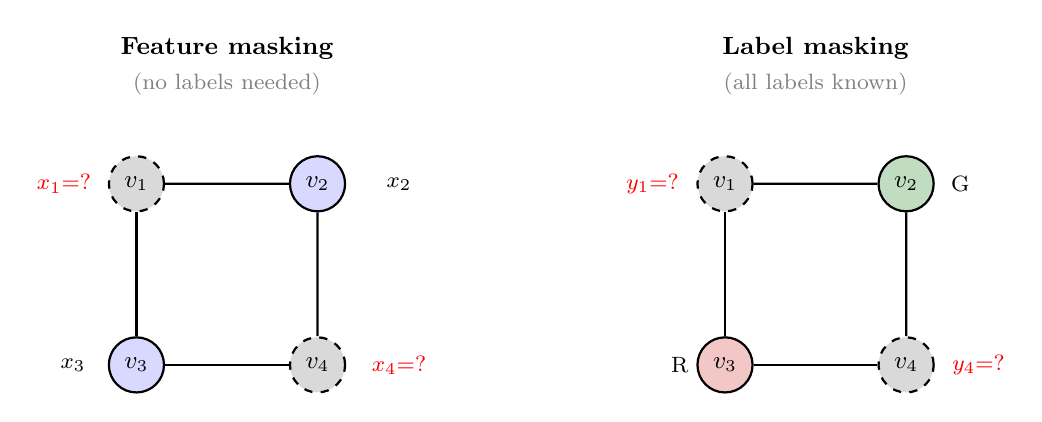
\begin{tikzpicture}[scale=1.15,
    node/.style={circle, draw, thick, minimum size=0.7cm, font=\small},
    masked/.style={circle, draw, thick, minimum size=0.7cm, font=\small,
      fill=gray!30, dashed}]

    % ---- LEFT: Feature masking (no labels needed) ----
    \begin{scope}[xshift=0cm]
        \node[draw=none, font=\small\bfseries] at (1,3.5)
          {Feature masking};
        \node[draw=none, font=\footnotesize, text=gray] at (1,3.1)
          {(no labels needed)};

        \node[masked] (a1) at (0,2) {$v_1$};
        \node[node, fill=blue!15] (a2) at (2,2) {$v_2$};
        \node[node, fill=blue!15] (a3) at (0,0) {$v_3$};
        \node[masked] (a4) at (2,0) {$v_4$};

        \draw[thick] (a1)--(a2); \draw[thick] (a1)--(a3);
        \draw[thick] (a2)--(a4); \draw[thick] (a3)--(a4);

        \node[draw=none, font=\footnotesize, text=red] at (-0.8,2) {$x_1{=}$?};
        \node[draw=none, font=\footnotesize] at (2.9,2) {$x_2$};
        \node[draw=none, font=\footnotesize] at (-0.7,0) {$x_3$};
        \node[draw=none, font=\footnotesize, text=red] at (2.9,0) {$x_4{=}$?};
    \end{scope}

    % ---- RIGHT: Label masking (fully-labeled pretraining data) ----
    \begin{scope}[xshift=6.5cm]
        \node[draw=none, font=\small\bfseries] at (1,3.5)
          {Label masking};
        \node[draw=none, font=\footnotesize, text=gray] at (1,3.1)
          {(all labels known)};

        \node[masked] (b1) at (0,2) {$v_1$};
        \node[node, fill=labeledgreen!30] (b2) at (2,2) {$v_2$};
        \node[node, fill=labeledred!30] (b3) at (0,0) {$v_3$};
        \node[masked] (b4) at (2,0) {$v_4$};

        \draw[thick] (b1)--(b2); \draw[thick] (b1)--(b3);
        \draw[thick] (b2)--(b4); \draw[thick] (b3)--(b4);

        \node[draw=none, font=\footnotesize, text=red] at (-0.8,2) {$y_1{=}$?};
        \node[draw=none, font=\footnotesize] at (2.6,2) {G};
        \node[draw=none, font=\footnotesize] at (-0.5,0) {R};
        \node[draw=none, font=\footnotesize, text=red] at (2.8,0) {$y_4{=}$?};
    \end{scope}
\end{tikzpicture}
\caption{Two variants of masked pretraining. Left: feature masking hides
  $x_1, x_4$ and trains the GNN to reconstruct them (no labels needed).
  Right: label masking hides $y_1, y_4$ and trains the GNN to predict them
  (requires a fully-labeled graph for pretraining). Gray dashed nodes are
  masked; the model must predict the ``?'' values from the remaining context.}
\label{semi-supervised-graphs:fig:masked_pretraining}
\end{figure}

\subsection{Mathematical Formulation}

Let $\mathcal{M} \subset V$ be a random mask with ratio
$p = |\mathcal{M}|/n$ (typically $0.15$--$0.30$).

\textbf{Feature masking objective.} Define the masked feature matrix
$\tilde{X}$ with $\tilde{X}_i = \mathbf{0}$ for $i \in \mathcal{M}$ and
$\tilde{X}_i = X_i$ otherwise. The pretraining loss is:
\begin{equation}
\label{semi-supervised-graphs:eq:feature_mask}
\mathcal{L}_{\text{feat}}(\theta) = \sum_{i \in \mathcal{M}}
  \|f_\theta(G, \tilde{X})_i - X_i\|^2
\end{equation}
To predict $X_i$, the GNN must aggregate information from $v_i$'s unmasked
neighbors via message passing---exactly the skill needed for downstream tasks.

\textbf{Label masking objective} (when a fully-labeled pretraining graph is
available). Define $\tilde{Y}$ with $\tilde{Y}_i = \mathbf{0}$ for
$i \in \mathcal{M}$ and $\tilde{Y}_i = Y_i$ otherwise. The GNN receives
both features $X$ and unmasked labels $\tilde{Y}$ as input:
\begin{equation}
\label{semi-supervised-graphs:eq:label_mask}
\mathcal{L}_{\text{label}}(\theta) = -\sum_{i \in \mathcal{M}} \sum_{c=1}^C
  Y_{ic}\,\log\bigl(f_\theta(G, X, \tilde{Y})_i\bigr)_c
\end{equation}
The unmasked labels are provided as input because we want the model to learn
how to \emph{propagate} label information across the graph---given some labels,
predict the rest. This directly simulates the semi-supervised scenario.

\subsection{The GPT-GNN Framework}

GPT-GNN~\cite{semi-supervised-graphs:hu2020} combines all three masking objectives into a unified
pretraining framework:
\begin{equation}
\mathcal{L}_{\text{GPT-GNN}} =
  \underbrace{\mathcal{L}_{\text{feat}}}_{\substack{\text{reconstruct}\\\text{masked features}}}
  + \underbrace{\mathcal{L}_{\text{edge}}}_{\substack{\text{predict}\\\text{masked edges}}}
  + \lambda\underbrace{\mathcal{L}_{\text{label}}}_{\substack{\text{predict}\\\text{masked labels}}}
\end{equation}
Each objective teaches a different skill: feature reconstruction teaches
neighborhood aggregation, edge prediction teaches topology awareness, and
label prediction teaches class propagation. The multi-task nature forces the
GNN to build representations that capture all aspects of the graph.

\subsection{Why Pretraining Helps: Intuition}

A randomly initialized GNN must simultaneously learn two things from the few
labeled nodes: (i) \emph{how} to aggregate neighborhood information
(the ``mechanics'' of message passing), and (ii) \emph{which} aggregated
patterns correspond to which classes. Pretraining separates these: the model
first learns (i) from the self-supervised task (which uses no labels), then
only needs to learn (ii) from the few downstream labels. This is easier
because the representation is already informative.

Recent theoretical work~\cite{semi-supervised-graphs:baranwal2023} formalizes this under a contextual
stochastic block model: masked pretraining provably learns a representation
that captures community structure, reducing the number of labeled examples
needed for downstream classification.

\subsection{Practical Implementation}

\begin{algorithm}[H]
\caption{Masked Feature Pretraining + Fine-tuning}
\label{semi-supervised-graphs:alg:masked_pretrain}
\begin{algorithmic}[1]
\State \textbf{Pretraining} (no labels used):
\For{each epoch}
    \State Sample mask $\mathcal{M} \subset V$, each node included
           independently with probability $p$
    \State Create $\tilde{X}$: set $\tilde{X}_i = \mathbf{0}$ for
           $i \in \mathcal{M}$, keep $\tilde{X}_i = X_i$ otherwise
    \State Forward pass: $\hat{X} = f_\theta(G, \tilde{X})$
    \State Loss: $\mathcal{L} = \sum_{i \in \mathcal{M}}
           \|\hat{X}_i - X_i\|^2$
    \State Update $\theta$ via gradient descent
\EndFor
\State
\State \textbf{Fine-tuning} (using the few available labels):
\State Initialize $f_\theta$ with pretrained weights
\State Replace reconstruction head with classification head
\State Train on labeled nodes with small learning rate (e.g., $10^{-3}$)
\end{algorithmic}
\end{algorithm}

\begin{warningbox}
\textbf{Implementation details:}
\begin{itemize}
    \item \textbf{Mask ratio.} Too low ($<0.1$): the task is too easy, the
          model learns little. Too high ($>0.5$): too little context remains.
          Typical range: $0.15$--$0.30$.
    \item \textbf{Fine-tuning learning rate.} Use a smaller learning rate
          than for pretraining (e.g., $10^{-3}$ vs.\ $10^{-2}$) to avoid
          destroying the pretrained representation.
    \item \textbf{Partial fine-tuning.} Freezing early GNN layers and only
          fine-tuning the classification head can help when very few labels
          are available.
\end{itemize}
\end{warningbox}

\subsection{Connection to Other Methods}

Self-supervised pretraining completes the progression of methods in this
document:

\textbf{Label propagation} propagates labels from fixed boundary nodes.
\textbf{Correct \& Smooth} propagates \emph{errors} from a base predictor.
\textbf{Graph regularization} adds graph smoothness as a training penalty.
\textbf{GNNs} learn to propagate and transform features end-to-end.
\textbf{Masked pretraining} teaches the GNN \emph{how} to aggregate
neighborhood information \emph{before} any labels are seen, providing a
better initialization for all GNN-based methods.

Self-supervised pretraining is not an alternative to GNNs---it is a way to
initialize them so that fine-tuning with few labels is more effective.

\section{Comparative Analysis and Guidelines}
\label{semi-supervised-graphs:sec:compare}

We have now seen five families of methods. They differ along several axes,
summarized in Table~\ref{semi-supervised-graphs:tab:comparison}.

\begin{table}[ht]
\centering\small
\begin{tabular}{lccccc}
\toprule
\textbf{Method} & \textbf{Uses Features} & \textbf{Inductive} &
\textbf{Scalability} & \textbf{Pretraining} & \textbf{Heterophily} \\ \midrule
Label Propagation & No & No & Medium & No & Poor \\
Label Spreading & No & No & Medium & No & Poor \\
Correct \& Smooth & Yes (via base) & No & High & No & Moderate \\
LapSVM & Yes & Yes & Low & No & Moderate \\
Neural Graph Learning & Yes & Yes & High & No & Moderate \\
GCN & Yes & Limited & Medium & No & Poor \\
GraphSAGE & Yes & Yes & High & No & Poor \\
GAT & Yes & Yes & Medium & No & Moderate \\
Masked Pretraining & Yes & Yes & Medium & Yes & Moderate \\
\bottomrule
\end{tabular}
\caption{Method comparison along key axes.}
\label{semi-supervised-graphs:tab:comparison}
\end{table}

\subsection{When to Use What}

\textbf{No node features available:}
Label propagation or label spreading. They require only the graph structure.
Correct \& Smooth is not applicable without a base predictor.

\textbf{Features available, small to medium graph ($n < 10^5$):}
Start with a 2-layer GCN---it's simple, fast, and often works well.
If you have a strong feature-based model (e.g., XGBoost on node features),
apply Correct \& Smooth to its predictions for a quick boost.

\textbf{Large graph ($n > 10^6$):}
GraphSAGE with neighbor sampling or Cluster-GCN. Full-batch GCN is infeasible.

\textbf{Inductive setting (unseen nodes at test time):}
GraphSAGE, GAT, neural graph learning, or masked pretraining + fine-tuning.
GCN is transductive unless combined with inductive extensions.

\textbf{Heterophilic graphs (low homophily):}
Test the homophily ratio first. If low, standard GCN and label propagation fail.
Consider H$_2$GCN~\cite{semi-supervised-graphs:zhu2020beyond}, LINKX~\cite{semi-supervised-graphs:lim2021large}, or
neural graph learning with feature-only base models.

\textbf{Very few labels ($l < 10$ per class):}
Self-supervised pretraining (Section~\ref{semi-supervised-graphs:sec:mlp}) can be very effective.
Pretrain on the same graph using feature masking (no extra labels needed),
then fine-tune. Alternatively, use label propagation or C\&S if the graph
has strong homophily.

\textbf{When you have abundant unlabeled data but limited labels:}
All methods will benefit, but Correct \& Smooth and graph regularization
explicitly leverage unlabeled nodes in the loss/optimization.

\subsection{Recommended Pipelines}

\begin{enumerate}
    \item \textbf{Quick baseline:} Train an MLP on node features (ignore graph).
          Apply Correct \& Smooth with $\alpha = \beta = 0.7$, 10 iterations
          each. This often beats fancy GNNs.

    \item \textbf{Standard transductive:} 2-layer GCN with hidden dimension 64,
          dropout 0.5, learning rate 0.01, trained for 200 epochs.

    \item \textbf{Standard inductive:} GraphSAGE with mean aggregator,
          neighbor samples [25, 10], hidden dimension 128, trained with
          mini-batches.

    \item \textbf{When you have abundant unlabeled features:} Masked feature
          pretraining (Section~\ref{semi-supervised-graphs:sec:mlp}) for 50--100 epochs, then
          fine-tune on target task with small learning rate.

    \item \textbf{When graph is heterophilic:} Use a feature-only MLP + C\&S,
          or specialized architectures like H$_2$GCN.
\end{enumerate}

\subsection{Key Hyperparameters}

\begin{itemize}
    \item \textbf{Label spreading:} $\alpha \in [0.5, 0.99]$, default 0.9.
    \item \textbf{Correct \& Smooth:} $\alpha = \beta \in [0.5, 0.9]$,
          iterations 5--20. Use asymmetric settings if correction needs to be
          stronger/weaker than smoothing.
    \item \textbf{GNNs:} 2--3 layers (more causes over-smoothing), hidden dim
          64--256, dropout 0.5--0.8, learning rate 0.001--0.01 with Adam.
    \item \textbf{GraphSAGE:} neighbor samples [25, 10] or [10, 5] for very
          large graphs.
    \item \textbf{GAT:} 8 attention heads in hidden layers, 1 in output,
          dropout 0.6.
    \item \textbf{Masked pretraining:} mask ratio 0.15--0.30,
          pretrain epochs 50--200, fine-tuning learning rate 0.001.
\end{itemize}

\section{Conclusion}

This document has presented a self-contained treatment of semi-supervised
learning on graphs, building from first principles to modern architectures
including the latest post-processing and pretraining methods. The unifying
thread is the graph Laplacian and its quadratic form
(Theorem~\ref{semi-supervised-graphs:thm:laplacian_quadratic}): every method in this document, from
label propagation to self-supervised pretraining, is connected to minimizing
$f^\top Lf$---the total variation of a signal across edges.

\textbf{Label propagation} (Section~\ref{semi-supervised-graphs:sec:lp}) is the simplest method: it
solves a discrete Dirichlet boundary value problem, finding the harmonic
function on unlabeled nodes that matches the given labels. Its convergence is
guaranteed by the sub-stochasticity of $P_{UU}$. Label spreading generalizes
this with soft clamping, providing robustness to label noise.

\textbf{Correct and Smooth} (Section~\ref{semi-supervised-graphs:sec:cs}) bridges the gap between
feature-based models and graph methods. It propagates errors from a base
predictor and then smooths the corrected predictions, achieving
state-of-the-art results with remarkable simplicity.

\textbf{Graph regularization} (Section~\ref{semi-supervised-graphs:sec:reg}) incorporates graph
structure into the loss function of parametric models, enabling classical
methods (kernel machines, neural networks) to leverage unlabeled data through
the manifold assumption.

\textbf{Graph neural networks} (Section~\ref{semi-supervised-graphs:sec:gnn}) encode graph structure
directly in the model architecture. The GCN layer is derived from spectral
graph theory; GraphSAGE enables inductive learning on large graphs; GAT
introduces learnable attention mechanisms.

\textbf{Self-supervised pretraining} (Section~\ref{semi-supervised-graphs:sec:mlp}) closes the loop
by teaching GNNs how to aggregate neighborhood information \emph{before} any
labels are seen. By masking node features (or, when available, labels) and
training the model to reconstruct them, pretraining provides a better
initialization that makes fine-tuning with few labels more effective.

All methods rest on the homophily assumption
(Assumption~\ref{semi-supervised-graphs:ass:smoothness})---the belief that connected nodes tend to
share labels. When this assumption fails (heterophilic graphs), specialized
architectures are required. Understanding when and why the homophily assumption
holds in a given application is perhaps the most important practical
consideration.

The field of semi-supervised graph learning continues to evolve rapidly, but
the mathematical foundations laid out in this document---spectral graph theory,
random walks, RKHS, diffusion processes---remain essential for understanding
both current methods and future innovations.


\chapterappendix
\newpage
\section{Extended Proofs}
\label{semi-supervised-graphs:app:proofs}

\subsection{Powers of a Matrix and the Spectral Radius
  (Proposition~\ref{semi-supervised-graphs:prop:spectral_powers})}
\label{semi-supervised-graphs:app:spectral_radius}

\begin{proof}
We prove $\rho(M) < 1 \implies M^t \to 0$. If $M$ is diagonalizable,
$M = Q\Lambda Q^{-1}$ where $\Lambda = \diag(\lambda_1, \ldots, \lambda_n)$.
Then $M^t = Q\Lambda^t Q^{-1}$, and $|\lambda_i|^t \leq \rho(M)^t \to 0$ since
$\rho(M) < 1$, so $M^t \to 0$.

For the general (non-diagonalizable) case, use the Jordan normal form
$M = QJQ^{-1}$. Each Jordan block of size $k$ with eigenvalue $\lambda$ has
entries $(J_\lambda^t)_{ij} = \binom{t}{j-i}\lambda^{t-(j-i)}$. Since
$|\lambda| < 1$, the geometric decay $|\lambda|^{t-\text{const}}$ dominates
the polynomial growth $\binom{t}{\text{const}}$, so each entry $\to 0$.
\end{proof}

\subsection{Sub-Stochasticity Implies $\rho(P_{UU})<1$ (Step~2 of
  Theorem~\ref{semi-supervised-graphs:thm:lp_closed})}
\label{semi-supervised-graphs:app:substochastic}

We prove that if $P_{UU}$ is sub-stochastic and $G$ is connected with at least
one labeled node, then $\rho(P_{UU}) < 1$.

\paragraph{Setup and intuition.}
Recall the block decomposition $P = \bigl(\begin{smallmatrix}P_{LL}&P_{LU}\\
P_{UL}&P_{UU}\end{smallmatrix}\bigr)$.  A random walker currently at unlabeled
node $v_i$ moves to node $v_j$ with probability $P_{ij}$.  If $v_j$ happens to
be a labeled node, the walk has \emph{escaped} $\mathcal{V}_U$.  Define
\[
  \ell_i \;:=\; \sum_{j \in \mathcal{V}_L} P_{ij}
  \;=\; 1 - \sum_{j \in \mathcal{V}_U}(P_{UU})_{ij} \;\geq\; 0,
\]
the \textbf{one-step escape probability} at $v_i$: the probability of jumping
directly into $\mathcal{V}_L$ in a single step.  By assumption, $\ell_i > 0$
for at least one unlabeled node (namely any node adjacent to a labeled node).

The key quantity we track is the \emph{total probability mass} that a
distribution $p \in \R^u$ (with $p_i \geq 0$, $\mathbf{1}^\top p = 1$) places
on $\mathcal{V}_U$ after repeated multiplication by $P_{UU}$.  At each step a
fraction $\ell_i$ of mass at node $v_i$ escapes; the total mass in
$\mathcal{V}_U$ can only decrease.

\paragraph{Proof.}
We use the following classical fact (a consequence of the Perron--Frobenius
theorem for non-negative matrices~\cite{semi-supervised-graphs:chung1997}):

\begin{quote}
\emph{For a non-negative matrix $B$, $\rho(B) < 1$ if and only if
$(I - B)$ is invertible and $(I-B)^{-1}$ has non-negative entries, i.e.\
$\sum_{t=0}^\infty B^t$ converges.}
\end{quote}

We establish $\rho(P_{UU}) < 1$ directly via the $\ell^\infty$ operator norm.

\begin{lemma}
Let $B \in \R^{u \times u}$ be non-negative with row sums
$r_i := \sum_j B_{ij} \leq 1$.  If $r_i < 1$ for at least one index $i_0$,
and $B$ is \emph{irreducible} (i.e.\ for every pair $(i,j)$ there exists $k$
such that $(B^k)_{ij} > 0$), then $\rho(B) < 1$.
\end{lemma}

\begin{proof}[Proof of Lemma]
\textbf{Step~A ($\|B\|_\infty \leq 1$).}
The $\ell^\infty$ operator norm of a non-negative matrix equals its maximum row
sum: $\|B\|_\infty = \max_i r_i \leq 1$.  Hence every eigenvalue satisfies
$|\lambda| \leq \|B\|_\infty \leq 1$, giving $\rho(B) \leq 1$.

\textbf{Step~B (ruling out $\rho(B) = 1$).}
Suppose for contradiction that $\rho(B)=1$, so there exists an eigenvalue
$\lambda$ with $|\lambda|=1$ and a corresponding eigenvector $v \neq 0$:
$Bv = \lambda v$.  Let $v_m$ be an entry of $v$ with maximum modulus:
$|v_m| = \|v\|_\infty$.  Then
\[
  |v_m| \;=\; |\lambda v_m| \;=\; |(Bv)_m|
  \;=\; \Bigl|\sum_j B_{mj} v_j\Bigr|
  \;\leq\; \sum_j B_{mj}|v_j|
  \;\leq\; \|v\|_\infty \sum_j B_{mj}
  \;=\; r_m \|v\|_\infty.
\]
Since $|v_m| = \|v\|_\infty$, we need $r_m \geq 1$.  But $r_m \leq 1$, so
$r_m = 1$ and equality holds throughout.  In particular, equality in the
triangle inequality forces all terms $B_{mj}v_j$ to point in the same complex
direction, and equality in the second step forces $|v_j| = \|v\|_\infty$
for every $j$ with $B_{mj} > 0$.

Iterating: the set $\mathcal{S} = \{i : |v_i| = \|v\|_\infty\}$ is closed
under the relation ``$B_{ij} > 0$''.  By irreducibility, starting from any
$m \in \mathcal{S}$ we can reach every index $j$, so $\mathcal{S} = \{1,
\ldots, u\}$.  But then, taking $i = i_0$ (where $r_{i_0} < 1$):
\[
  |v_{i_0}| \;\leq\; r_{i_0}\|v\|_\infty \;<\; \|v\|_\infty,
\]
contradicting $i_0 \in \mathcal{S}$.  Hence $\rho(B) < 1$.
\end{proof}

\paragraph{Applying the lemma to $P_{UU}$.}
We verify the two hypotheses:
\begin{enumerate}
  \item \emph{Row sums $\leq 1$ with at least one strict.}
    By definition, $(P_{UU})_{ij} = P_{ij}$ for $i,j \in \mathcal{V}_U$, and
    $\sum_{j \in \mathcal{V}_U}(P_{UU})_{ij} = 1 - \ell_i \leq 1$.  Since $G$
    contains at least one edge between $\mathcal{V}_U$ and $\mathcal{V}_L$,
    some node $i_0 \in \mathcal{V}_U$ has $\ell_{i_0} > 0$, giving a strictly
    sub-unit row sum.
  \item \emph{Irreducibility.}
    Since $G$ is connected, every pair of unlabeled nodes is connected by a
    path in $G$.  Any edge $\{i,j\}$ in $G$ with $i,j \in \mathcal{V}_U$
    contributes $(P_{UU})_{ij} = A_{ij}/d_i > 0$.  Hence for every $i,j \in
    \mathcal{V}_U$ there exists $k$ such that $(P_{UU}^k)_{ij} > 0$, i.e.\
    $P_{UU}$ is irreducible.
\end{enumerate}
The lemma therefore gives $\rho(P_{UU}) < 1$, and $I - P_{UU}$ is invertible.
\qed

\subsection{Proof of the Representer Theorem (Theorem~\ref{semi-supervised-graphs:thm:representer})}
\label{semi-supervised-graphs:app:representer}

\begin{proof}
Decompose $f \in \mathcal{H}_K$ as $f = f_\parallel + f_\perp$ where
$f_\parallel = \sum_{i=1}^n \alpha_i K(\cdot, x_i)$ lies in
$\text{span}\{K(\cdot, x_1), \ldots, K(\cdot, x_n)\}$ and $f_\perp$ is
orthogonal to this span.

By the reproducing property,
$f(x_i) = \inner{f}{K(\cdot, x_i)}_{\mathcal{H}_K}
= \inner{f_\parallel}{K(\cdot, x_i)} + \inner{f_\perp}{K(\cdot, x_i)}
= f_\parallel(x_i)$ since $f_\perp \perp K(\cdot, x_i)$.

So the loss $\sum_i \ell(f(x_i), y_i) = \sum_i \ell(f_\parallel(x_i), y_i)$
depends only on $f_\parallel$.

For the regularizer: $\|f\|^2 = \|f_\parallel\|^2 + \|f_\perp\|^2
\geq \|f_\parallel\|^2$, with equality iff $f_\perp = 0$.

Therefore $f^* = f_\parallel^*$ (setting $f_\perp = 0$ can only decrease the
objective), giving $f^*(x) = \sum_{i=1}^n \alpha_i K(x, x_i)$.

\textbf{RKHS norm of the solution.} For $f^* = \sum_i \alpha_i K(\cdot, x_i)$:
\begin{align}
\|f^*\|_{\mathcal{H}_K}^2 &=
\inner{\sum_i \alpha_i K(\cdot, x_i)}{\sum_j \alpha_j K(\cdot, x_j)}_{
\mathcal{H}_K} \\
&= \sum_{i,j}\alpha_i\alpha_j \underbrace{\inner{K(\cdot, x_i)}{K(\cdot, x_j)}_{
\mathcal{H}_K}}_{= K(x_i, x_j) \text{ (reproducing property)}} \\
&= \sum_{i,j}\alpha_i\alpha_j K(x_i, x_j) = \boldsymbol{\alpha}^\top
\mathbf{K}\boldsymbol{\alpha}
\end{align}
This identity is used in Remark~\ref{semi-supervised-graphs:rem:rkhs_practical} to kernelize the
objective.
\end{proof}

\subsection{Proof of the Variational Formulation (Theorem~\ref{semi-supervised-graphs:thm:ls_energy})}
\label{semi-supervised-graphs:app:ls_energy}

\begin{proof}
Working with a single class column $f \in \R^n$ and initial labels
$y^{(0)}$:
\begin{equation}
\mathcal{E}(f) = f^\top(I - S)f + \frac{1-\alpha}{\alpha}\|f - y^{(0)}\|^2
\end{equation}

The first term uses $\sum_{\{i,j\}\in E}A_{ij}\bigl(\frac{f_i}{\sqrt{d_i}} -
\frac{f_j}{\sqrt{d_j}}\bigr)^2 = f^\top\mathcal{L}_{\mathrm{sym}}f
= f^\top(I-S)f$ (this is the normalized analogue of
Theorem~\ref{semi-supervised-graphs:thm:laplacian_quadratic}, proved by setting $g_i = f_i/\sqrt{d_i}$
and applying the unnormalized form to $g$).

Taking the gradient and setting it to zero:
\begin{align}
\nabla_f \mathcal{E} &= 2(I - S)f + \frac{2(1-\alpha)}{\alpha}(f - y^{(0)}) = 0\\
(I - S)f + \frac{1-\alpha}{\alpha}f &= \frac{1-\alpha}{\alpha}y^{(0)} \\
\frac{1}{\alpha}f - Sf &= \frac{1-\alpha}{\alpha}y^{(0)} \\
f &= \alpha Sf + (1-\alpha)y^{(0)}
\end{align}
This is the label spreading fixed point. The Hessian is
$2(I - S) + \frac{2(1-\alpha)}{\alpha}I = \frac{2}{\alpha}I - 2S$, which is
positive definite (eigenvalues $\frac{2}{\alpha} - 2\sigma_k > 0$ since
$\sigma_k \leq 1$ and $\alpha < 1$). So the critical point is a global minimum.
\end{proof}

\subsection{Proofs of C\&S Variational Theorems
  (Theorems~\ref{semi-supervised-graphs:thm:cs_correct_opt} and~\ref{semi-supervised-graphs:thm:cs_smooth_opt})}
\label{semi-supervised-graphs:app:cs_opt}

Both theorems are instances of the same general result.

\begin{proof}[Proof of the general template~\eqref{semi-supervised-graphs:eq:cs_general_opt}]
Working column by column (the $C$ columns decouple), it suffices to prove the
scalar case: minimize over $f \in \R^n$
\[
  \mathcal{E}(f) = \|f - b\|^2 + \mu\sum_{i,j}A_{ij}
  \left(\frac{f_i}{\sqrt{d_i}} - \frac{f_j}{\sqrt{d_j}}\right)^2.
\]
\textbf{Rewriting the smoothness term.}
By the normalized analogue of Theorem~\ref{semi-supervised-graphs:thm:laplacian_quadratic} (proved by
setting $g_i = f_i/\sqrt{d_i}$ and applying the unnormalized form to $g$):
\[
\frac{1}{2}\sum_{i,j}A_{ij}\left(\frac{f_i}{\sqrt{d_i}} -
\frac{f_j}{\sqrt{d_j}}\right)^2
= g^\top L g = f^\top D^{-1/2}LD^{-1/2}f = f^\top\mathcal{L}_{\mathrm{sym}}f
= f^\top(I-S)f,
\]
where $g = D^{-1/2}f$. The full sum (without the $\frac{1}{2}$) equals
$2f^\top(I-S)f$. Hence:
\[
\mathcal{E}(f) = \|f - b\|^2 + 2\mu\, f^\top(I-S)f.
\]

\textbf{Minimizing.} Setting the gradient to zero:
\begin{align}
\nabla_f\mathcal{E} &= 2(f - b) + 4\mu(I - S)f = 0 \notag\\
((1+2\mu)I - 2\mu S)\,f &= b. \label{semi-supervised-graphs:eq:cs_normal}
\end{align}
Define $\alpha := 1/(1+2\mu)$, so that $2\mu = (1-\alpha)/\alpha$ and
$(1+2\mu) = 1/\alpha$. Multiplying~\eqref{semi-supervised-graphs:eq:cs_normal} through by $\alpha$:
\[
(I - \alpha S)\,f = \alpha b,
\]
giving the unique minimizer:
\begin{equation}
\label{semi-supervised-graphs:eq:cs_solution}
f^* = \alpha(I - \alpha S)^{-1}b.
\end{equation}
Invertibility of $I - \alpha S$ follows from $\rho(\alpha S) \leq \alpha < 1$,
exactly as in Theorem~\ref{semi-supervised-graphs:thm:ls_closed}.

\textbf{Connection to the theorem statements.}
In Theorems~\ref{semi-supervised-graphs:thm:cs_correct_opt} and~\ref{semi-supervised-graphs:thm:cs_smooth_opt}, the
smoothness coefficient is $\alpha/(1-\alpha)$, corresponding to
$\mu = \alpha/(2(1-\alpha))$, so~\eqref{semi-supervised-graphs:eq:cs_solution} applies directly.
The closed forms stated in the C\&S algorithm use the label-spreading
convention $(1-\alpha)(I-\alpha S)^{-1}B$: this is obtained by absorbing the
scalar $\alpha$ into the target $b' = \alpha b/(1-\alpha)$ and writing the
solution as $(1-\alpha)(I-\alpha S)^{-1}b'$. Both forms are equivalent up to
this rescaling of $b$; the important point is the unique minimizer~\eqref{semi-supervised-graphs:eq:cs_solution}.

\textbf{Uniqueness (Hessian is positive definite).}
\[
H = \nabla^2_f \mathcal{E} = 2I + 4\mu(I - S).
\]
Since $I - S = \mathcal{L}_{\mathrm{sym}} \succeq 0$
(Proposition~\ref{semi-supervised-graphs:prop:normalized_properties}) and $\mu > 0$, the eigenvalues
of $H$ are $\geq 2 > 0$, so $H \succ 0$ and the critical point is the unique
global minimum.
\end{proof}

Theorem~\ref{semi-supervised-graphs:thm:cs_correct_opt} follows by taking $b = E$ and
$\mu = \alpha/(2(1-\alpha))$. Theorem~\ref{semi-supervised-graphs:thm:cs_smooth_opt} follows by
taking $b = \hat{Y}^{\text{corr}}$ and $\mu = \beta/(2(1-\beta))$.

\subsection{GCN Layer Derivation (Theorem~\ref{semi-supervised-graphs:thm:gcn})}
\label{semi-supervised-graphs:app:gcn_derivation}

\begin{proof}[Derivation]
We carry out the derivation in four steps: ChebNet approximation, Kipf \&
Welling's first-order simplification, renormalization, and the generalization
from a single filtered signal to the full layer update $H^{(k+1)}$.

\textbf{Step 1: ChebNet approximation.}
ChebNet~\cite{semi-supervised-graphs:defferrard2016} avoids the $O(n^3)$ eigendecomposition by
approximating the spectral filter $g_\theta(\Lambda)$ with a degree-$K$
Chebyshev polynomial:
\[
g_\theta(\Lambda) \approx \sum_{k=0}^K \theta_k T_k(\tilde{\Lambda}), \qquad
\tilde{\Lambda} = \tfrac{2}{\lambda_{\max}}\Lambda - I,
\]
where the rescaling maps eigenvalues from $[0, \lambda_{\max}]$ to $[-1,1]$,
the natural domain of Chebyshev polynomials. Since $T_k$ is a polynomial,
$U T_k(\tilde\Lambda) U^\top = T_k(\tilde{\mathcal{L}}_{\mathrm{sym}})$ where
$\tilde{\mathcal{L}}_{\mathrm{sym}} = \frac{2}{\lambda_{\max}}\mathcal{L}_{\mathrm{sym}}
- I$. The convolution becomes:
\[
g_\theta \star x = \sum_{k=0}^K \theta_k\, T_k(\tilde{\mathcal{L}}_{\mathrm{sym}})\,x,
\]
which requires only sparse matrix-vector products (cost $O(K|E|)$, no
eigenvectors needed).

\textbf{Step 2: First-order simplification ($K=1$, $\lambda_{\max} \approx 2$).}
Setting $K=1$ and $\lambda_{\max} \approx 2$ gives
$\tilde{\mathcal{L}}_{\mathrm{sym}} = \mathcal{L}_{\mathrm{sym}} - I
= -D^{-1/2}AD^{-1/2}$ (since $\mathcal{L}_{\mathrm{sym}} = I - D^{-1/2}AD^{-1/2}$),
and $T_0(\cdot) = 1$, $T_1(\cdot) = \text{id}$:
\[
g_\theta \star x \approx \theta_0\,x + \theta_1\,\tilde{\mathcal{L}}_{\mathrm{sym}}\,x
= \theta_0\,x - \theta_1\,D^{-1/2}AD^{-1/2}\,x.
\]
Constraining to a single free parameter $\theta_0 = -\theta_1 =: \theta$
reduces overfitting:
\[
g_\theta \star x = \theta\,(I + D^{-1/2}AD^{-1/2})\,x.
\]

\textbf{Step 3: Renormalization trick.}
The matrix $I + D^{-1/2}AD^{-1/2}$ has eigenvalues in $[0, 2]$ (since
$D^{-1/2}AD^{-1/2}$ has eigenvalues in $[-1, 1]$ by
Proposition~\ref{semi-supervised-graphs:prop:normalized_properties}). Eigenvalues near $2$ cause
numerical instability when stacking multiple layers. Kipf \& Welling replace
this matrix with the renormalized version using $\tilde{A} = A + I$
(adding self-loops) and $\tilde{D}_{ii} = \sum_j \tilde{A}_{ij} = d_i + 1$:
\[
\hat{A} := \tilde{D}^{-1/2}\tilde{A}\tilde{D}^{-1/2}.
\]
Since $\tilde{A}$ is the adjacency of a graph with self-loops added, its
normalized version $\hat{A}$ has eigenvalues in $[0, 1]$ (approximately),
stabilizing repeated multiplication across layers. The filtered signal is now:
\[
g_\theta \star x \approx \theta\,\hat{A}\,x.
\]

\textbf{Step 4: From a single filtered signal to the layer update $H^{(k+1)}$.}
So far, $x \in \R^n$ is a single scalar signal on the graph (one feature
channel) and $\theta \in \R$ is a single learnable scalar. In practice, each
node carries a $d_k$-dimensional feature vector, so the input to layer $k$ is
a \textbf{feature matrix} $H^{(k)} \in \R^{n \times d_k}$, where row $i$ is
the representation of node $v_i$.

We apply the filtered convolution to each of the $d_k$ input channels
independently, then mix the results into $d_{k+1}$ output channels via a
learnable linear map. Specifically, let $W^{(k)} \in \R^{d_k \times d_{k+1}}$
be the weight matrix for layer $k$. Applying $\hat{A}$ to every column of
$H^{(k)}$ simultaneously:
\[
\hat{A}\,H^{(k)} \in \R^{n \times d_k},
\]
where row $i$ is $\sum_{j} \hat{A}_{ij}\,h_j^{(k)}$, the normalized weighted
average of node $v_i$'s neighbors' (and its own) representations. Then the
linear mixing $(\hat{A}H^{(k)})W^{(k)}$ produces an $n \times d_{k+1}$ matrix
of pre-activations. Applying a nonlinearity $\sigma$ element-wise gives:
\[
H^{(k+1)} = \sigma\!\bigl(\hat{A}\,H^{(k)}\,W^{(k)}\bigr) \in \R^{n \times d_{k+1}}.
\]
This is the GCN layer formula of Theorem~\ref{semi-supervised-graphs:thm:gcn}. The scalar filter
parameter $\theta$ has been absorbed into $W^{(k)}$: where before we had a
single scalar multiplying $\hat{A}x$, now $W^{(k)}$ is a full matrix
performing a learnable linear combination of the $d_k$ filtered channels into
$d_{k+1}$ output channels. The initial input is $H^{(0)} = X \in \R^{n \times d}$,
the raw node feature matrix.
\end{proof}

\subsection{Manifold Regularization Representer Theorem
  (Theorem~\ref{semi-supervised-graphs:thm:manifold_reg})}
\label{semi-supervised-graphs:app:manifold}

\begin{proof}
The key extension is showing $\mathbf{f}^\top L\mathbf{f}$ depends only on
$f_\parallel$. Since $f(x_i) = f_\parallel(x_i)$ (same argument as
Appendix~\ref{semi-supervised-graphs:app:representer}), we have $\mathbf{f} = \mathbf{f}_\parallel$,
so $\mathbf{f}^\top L\mathbf{f} = \mathbf{f}_\parallel^\top L\mathbf{f}_\parallel$.
The full objective therefore depends only on $f_\parallel$, and minimizing over
$f_\perp$ again gives $f_\perp^* = 0$. Substituting
$f^*(x) = \sum_i \alpha_i K(x, x_i)$ yields $\mathbf{f}^* = K\boldsymbol{\alpha}$
and the objective becomes a finite-dimensional problem in
$\boldsymbol{\alpha} \in \R^n$.
\end{proof}


\newpage
\section{Python Code for Numerical Examples}
\label{semi-supervised-graphs:app:code}

The following script reproduces the Correct \& Smooth numerical example of
Section~\ref{semi-supervised-graphs:sec:cs}. It constructs the 5-node graph, computes the normalized
adjacency~$S$, runs the correction and smoothing iterations, and prints the
table values used in the text.


\begin{tcolorbox}[
  title={Listing 1: Correct \& Smooth on the 5-node example (Section~\ref{semi-supervised-graphs:sec:cs})},
  colback=white, colframe=black!70, fonttitle=\small\bfseries,
  breakable, enhanced, left=2mm, right=2mm, top=1mm, bottom=1mm]
\begin{lstlisting}[language=Python, basicstyle=\ttfamily\small]
import numpy as np

# --- Graph -----------------------------------------------------------
# Edges: v1-v3, v1-v4, v2-v4, v2-v5, v3-v4 (unweighted)
# Indices: 0=v1, 1=v2, 2=v3, 3=v4, 4=v5
A = np.array([[0,0,1,1,0],
              [0,0,0,1,1],
              [1,0,0,1,0],
              [1,1,1,0,0],
              [0,1,0,0,0]], dtype=float)
d = A.sum(axis=1)                         # degrees: [2,2,2,3,1]
D_inv_sqrt = np.diag(1.0 / np.sqrt(d))
S = D_inv_sqrt @ A @ D_inv_sqrt           # normalized adjacency

# --- Base predictions and errors -------------------------------------
Y_hat = np.array([[0.70, 0.30],           # v1
                  [0.40, 0.60],           # v2
                  [0.60, 0.40],           # v3
                  [0.55, 0.45],           # v4
                  [0.45, 0.55]])          # v5
Y_true = np.array([[1,0],                 # v1 = Red
                   [0,1],                 # v2 = Green
                   [0,0],[0,0],[0,0]])    # unlabeled
E = np.zeros_like(Y_hat)
E[0] = Y_true[0] - Y_hat[0]              # [+0.3, -0.3]
E[1] = Y_true[1] - Y_hat[1]              # [-0.4, +0.4]

# --- Stage 1: Correct -----------------------------------------------
alpha = 0.7
E_star = E.copy()
for _ in range(50):
    E_star = (1 - alpha) * E + alpha * S @ E_star

Y_corr = Y_hat + E_star
Y_corr[0] = [1, 0]                       # clamp labeled
Y_corr[1] = [0, 1]

# --- Stage 2: Smooth ------------------------------------------------
beta = 0.7
Z = Y_corr.copy()
for _ in range(50):
    Z = (1 - beta) * Y_corr + beta * S @ Z

Z_norm = Z / Z.sum(axis=1, keepdims=True) # row-normalize

# --- Print results ---------------------------------------------------
header = f"{'Node':>6} {'Base':>14} {'E*':>14} " \
         f"{'Corrected':>14} {'Smoothed':>14}"
print(header)
names = ['v1(R)', 'v2(G)', 'v3', 'v4', 'v5']
for i in range(5):
    b = f"[{Y_hat[i,0]:.2f}, {Y_hat[i,1]:.2f}]"
    e = f"[{E_star[i,0]:+.3f},{E_star[i,1]:+.3f}]" \
        if i >= 2 else "   (labeled)  "
    c = f"[{Y_corr[i,0]:.2f}, {Y_corr[i,1]:.2f}]"
    s = f"[{Z_norm[i,0]:.2f}, {Z_norm[i,1]:.2f}]"
    print(f"{names[i]:>6} {b:>14} {e:>14} {c:>14} {s:>14}")
\end{lstlisting}
\end{tcolorbox}

\noindent\textbf{Expected output:}
\begin{tcolorbox}[colback=black!3, colframe=black!40, left=2mm, right=2mm,
  top=1mm, bottom=1mm]
\begin{verbatim}
  Node     Base            E*        Corrected     Smoothed
 v1(R)  [0.70, 0.30]    (labeled)    [1.00, 0.00] [0.72, 0.28]
 v2(G)  [0.40, 0.60]    (labeled)    [0.00, 1.00] [0.30, 0.70]
    v3  [0.60, 0.40] [+0.032,-0.032] [0.63, 0.37] [0.63, 0.37]
    v4  [0.55, 0.45] [-0.009,+0.009] [0.54, 0.46] [0.54, 0.46]
    v5  [0.45, 0.55] [-0.080,+0.080] [0.37, 0.63] [0.33, 0.67]
\end{verbatim}
\end{tcolorbox}

\newpage
\bibliographystyle{plain}
\begin{thebibliography}{99}

\bibitem{semi-supervised-graphs:zhu2002}
X. Zhu and Z. Ghahramani.
\textit{Learning from Labeled and Unlabeled Data with Label Propagation}.
Technical Report CMU-CALD-02-107, Carnegie Mellon University, 2002.

\bibitem{semi-supervised-graphs:zhou2004}
D. Zhou, O. Bousquet, T. Lal, J. Weston, and B. Sch\"{o}lkopf.
\textit{Learning with Local and Global Consistency}.
NeurIPS, 2004.

\bibitem{semi-supervised-graphs:huang2021}
Q. Huang, H. He, A. Singh, S. Lim, and A. R. Benson.
\textit{Combining Label Propagation and Simple Models Out-performs Graph Neural Networks}.
ICLR, 2021.

\bibitem{semi-supervised-graphs:belkin2006}
M. Belkin, P. Niyogi, and V. Sindhwani.
\textit{Manifold Regularization: A Geometric Framework for Learning from
  Labeled and Unlabeled Examples}.
JMLR, 7:2399--2434, 2006.

\bibitem{semi-supervised-graphs:scholkopf2001}
B. Sch\"{o}lkopf, R. Herbrich, and A. J. Smola.
\textit{A Generalized Representer Theorem}.
COLT, 2001.

\bibitem{semi-supervised-graphs:bui2018}
T. Bui, S. Ravi, and V. Ramavajjala.
\textit{Neural Graph Learning: Training Neural Networks Using Graphs}.
WSDM, 2018.

\bibitem{semi-supervised-graphs:kipf2017}
T. N. Kipf and M. Welling.
\textit{Semi-Supervised Classification with Graph Convolutional Networks}.
ICLR, 2017.

\bibitem{semi-supervised-graphs:defferrard2016}
M. Defferrard, X. Bresson, and P. Vandergheynst.
\textit{Convolutional Neural Networks on Graphs with Fast Localized Spectral
  Filtering}.
NeurIPS, 2016.

\bibitem{semi-supervised-graphs:hamilton2017}
W. L. Hamilton, Z. Ying, and J. Leskovec.
\textit{Inductive Representation Learning on Large Graphs}.
NeurIPS, 2017.

\bibitem{semi-supervised-graphs:velivckovic2018}
P. Veli\v{c}kovi\'{c}, G. Cucurull, A. Casanova, A. Romero, P. Li\`{o},
  and Y. Bengio.
\textit{Graph Attention Networks}.
ICLR, 2018.

\bibitem{semi-supervised-graphs:gilmer2017}
J. Gilmer, S. S. Schoenholz, P. F. Riley, O. Vinyals, and G. E. Dahl.
\textit{Neural Message Passing for Quantum Chemistry}.
ICML, 2017.

\bibitem{semi-supervised-graphs:hu2020}
W. Hu et al.
\textit{GPT-GNN: Generative Pre-Training of Graph Neural Networks}.
KDD, 2020.

\bibitem{semi-supervised-graphs:baranwal2023}
A. Baranwal, K. Fountoulakis, and A. Jagannath.
\textit{Why Pretraining Works on Graph Neural Networks: A Theoretical Perspective}.
arXiv:2302.11945, 2023.

\bibitem{semi-supervised-graphs:chung1997}
F. R. K. Chung.
\textit{Spectral Graph Theory}.
AMS, 1997.

\bibitem{semi-supervised-graphs:zhang2021magnet}
X. Zhang, Y. He, N. Brugnone, M. Perlmutter, and M. Hirn.
\textit{MagNet: A Neural Network for Directed Graphs}.
NeurIPS, 2021.

\bibitem{semi-supervised-graphs:li2018deeper}
Q. Li, Z. Han, and X.-M. Wu.
\textit{Deeper Insights into Graph Convolutional Networks for Semi-Supervised
  Learning}.
AAAI, 2018.

\bibitem{semi-supervised-graphs:xu2018representation}
K. Xu, C. Li, Y. Tian, T. Sonobe, K. Kawarabayashi, and S. Jegelka.
\textit{Representation Learning on Graphs with Jumping Knowledge Networks}.
ICML, 2018.

\bibitem{semi-supervised-graphs:rong2020dropedge}
Y. Rong, W. Huang, T. Xu, and J. Huang.
\textit{DropEdge: Towards Deep Graph Convolutional Networks on Node
  Classification}.
ICLR, 2020.

\bibitem{semi-supervised-graphs:zhao2020pairnorm}
L. Zhao and L. Akoglu.
\textit{PairNorm: Tackling Oversmoothing in GNNs}.
ICLR, 2020.

\bibitem{semi-supervised-graphs:ying2021transformers}
C. Ying et al.
\textit{Do Transformers Really Perform Bad for Graph Representation?}
NeurIPS, 2021.

\bibitem{semi-supervised-graphs:chiang2019cluster}
W.-L. Chiang et al.
\textit{Cluster-GCN: An Efficient Algorithm for Training Deep and Large Graph
  Convolutional Networks}.
KDD, 2019.

\bibitem{semi-supervised-graphs:zhu2020beyond}
J. Zhu et al.
\textit{Beyond Homophily in Graph Neural Networks: Current Limitations and
  Effective Designs}.
NeurIPS, 2020.

\bibitem{semi-supervised-graphs:lim2021large}
D. Lim et al.
\textit{Large Scale Learning on Non-Homophilous Graphs: New Benchmarks and
  Strong Simple Methods}.
NeurIPS, 2021.

\bibitem{semi-supervised-graphs:bronstein2017}
M. M. Bronstein, J. Bruna, Y. LeCun, A. Szlam, and P. Vandergheynst.
\textit{Geometric Deep Learning: Going Beyond Euclidean Data}.
IEEE Signal Processing Magazine, 34(4):18--42, 2017.

\end{thebibliography}
\end{notechapter}
